%% This is file `elsarticle-template-1-num.tex',
%%
%% Copyright 2009 Elsevier Ltd
%%
%% This file is part of the 'Elsarticle Bundle'.
%% ---------------------------------------------
%%
%% It may be distributed under the conditions of the LaTeX Project Public
%% License, either version 1.2 of this license or (at your option) any
%% later version.  The latest version of this license is in
%%    http://www.latex-project.org/lppl.txt
%% and version 1.2 or later is part of all distributions of LaTeX
%% version 1999/12/01 or later.
%%
%% The list of all files belonging to the 'Elsarticle Bundle' is
%% given in the file `manifest.txt'.
%%
%% Template article for Elsevier's document class `elsarticle'
%% with numbered style bibliographic references
%%
%% $Id: elsarticle-template-1-num.tex 149 2009-10-08 05:01:15Z rishi $
%% $URL: http://lenova.river-valley.com/svn/elsbst/trunk/elsarticle-template-1-num.tex $
%%
\documentclass[preprint,12pt]{elsarticle}

%% Use the option review to obtain double line spacing
%% \documentclass[preprint,review,12pt]{elsarticle}

%% Use the options 1p,twocolumn; 3p; 3p,twocolumn; 5p; or 5p,twocolumn
%% for a journal layout:
%% \documentclass[final,1p,times]{elsarticle}
%% \documentclass[final,1p,times,twocolumn]{elsarticle}
%% \documentclass[final,3p,times]{elsarticle}
%% \documentclass[final,3p,times,twocolumn]{elsarticle}
%% \documentclass[final,5p,times]{elsarticle}
%% \documentclass[final,5p,times,twocolumn]{elsarticle}

%% if you use PostScript figures in your article
%% use the graphics package for simple commands
%% \usepackage{graphics}
%% or use the graphicx package for more complicated commands
%% \usepackage{graphicx}
%% or use the epsfig package if you prefer to use the old commands
%% \usepackage{epsfig}

%% The amssymb package provides various useful mathematical symbols
\usepackage{amssymb}
\usepackage{amsmath}
\usepackage{color}
\usepackage{listings} % for listing code
\usepackage{etoolbox} % for toggles
\usepackage[colorlinks]{hyperref}

%% Send all the pictures to the end of the document
\usepackage[nolists, nomarkers]{endfloat}

%% The amsthm package provides extended theorem environments
%% \usepackage{amsthm}

%% The lineno packages adds line numbers. Start line numbering with
%% \begin{linenumbers}, end it with \end{linenumbers}. Or switch it on
%% for the whole article with \linenumbers after \end{frontmatter}.
%% \usepackage{lineno}

%% natbib.sty is loaded by default. However, natbib options can be
%% provided with \biboptions{...} command. Following options are
%% valid:

%%   round  -  round parentheses are used (default)
%%   square -  square brackets are used   [option]
%%   curly  -  curly braces are used      {option}
%%   angle  -  angle brackets are used    <option>
%%   semicolon  -  multiple citations separated by semi-colon
%%   colon  - same as semicolon, an earlier confusion
%%   comma  -  separated by comma
%%   numbers-  selects numerical citations
%%   super  -  numerical citations as superscripts
%%   sort   -  sorts multiple citations according to order in ref. list
%%   sort&compress   -  like sort, but also compresses numerical citations
%%   compress - compresses without sorting
%%
%% \biboptions{comma,round}

% \biboptions{}
%%---------------------------------------------------------------------------%%
%% DEFINE SPECIFIC ENVIRONMENTS HERE
%%---------------------------------------------------------------------------%%
% Mark URL's
\newcommand{\URL}[1]{{\textcolor{blue}{#1}}}

%\newcommand{\elfit}{\ensuremath{\operatorname{Im}(-1/\epsilon(\vq,\omega)}}
%\msection{}-->section commands
%\tradem{}  -->add TM subscript to entry
%\ucatm{}   -->add trademark footnote about entry
%
% Ways of grouping things
%
\newcommand{\bracket}[1]{\left[ #1 \right]}
\newcommand{\bracet}[1]{\left\{ #1 \right\}}
\newcommand{\fn}[1]{\left( #1 \right)}
\newcommand{\ave}[1]{\left\langle #1 \right\rangle}
\newcommand{\norm}[1]{\Arrowvert #1 \Arrowvert}
\newcommand{\abs}[1]{\arrowvert #1 \arrowvert}

%
% Derivative forms
%
%\newcommand{\dx}[1]{\,d#1}
\newcommand{\dxdy}[2]{\frac{\partial #1}{\partial #2}}
\newcommand{\dxy}[2]{\frac{d #1}{d #2}}
\newcommand{\dxdt}[1]{\frac{\partial #1}{\partial t}}
\newcommand{\dydt}[1]{\frac{\partial #1}{\partial t}}
\newcommand{\dxdz}[1]{\frac{\partial #1}{\partial z}}
\newcommand{\dfdt}[1]{\frac{\partial}{\partial t} \fn{#1}}
\newcommand{\dfdz}[1]{\frac{\partial}{\partial z} \fn{#1}}
\newcommand{\ddt}[1]{\frac{\partial}{\partial t} #1}
\newcommand{\ddz}[1]{\frac{\partial}{\partial z} #1}
\newcommand{\dd}[2]{\frac{\partial}{\partial #1} #2}
\newcommand{\ddx}[1]{\frac{\partial}{\partial x} #1}
\newcommand{\ddy}[1]{\frac{\partial}{\partial y} #1}
\newcommand{\dxdyn}[3]{\frac{\partial ^{#3} #1 }{\partial #2 ^{#3}}}
\newcommand{\Dxdy}[2]{\frac{D #1}{D #2}}
\newcommand{\Dxy}[2]{\frac{D #1}{D #2}}
%
% Vector forms
%
\renewcommand{\vec}[1]{\mbox{$\stackrel{\longrightarrow}{#1}$}}
\renewcommand{\div}{\mbox{$\vec{\nabla} \cdot$}}
\newcommand{\grad}{\mbox{$\vec{\nabla}$}}
\newcommand{\bb}[1]{\bar{\bar{#1}}}
%
% Equation beginnings and endings
%
\newcommand{\bea}{\begin{eqnarray}}
\newcommand{\eea}{\end{eqnarray}}
\newcommand{\be}{\begin{equation}}
\newcommand{\ee}{\end{equation}}
\newcommand{\beas}{\begin{eqnarray*}}
\newcommand{\eeas}{\end{eqnarray*}}
\newcommand{\bdm}{\begin{displaymath}}
\newcommand{\edm}{\end{displaymath}}
%
% Equation punctuation
%
\newcommand{\pec}{\, ,}
\newcommand{\pep}{\, .} 
\newcommand{\pev}{\hspace{0.25in}}
%
% Equation labels and references, figure references, table references
%
\newcommand{\LEQ}[1]{\label{eq:#1}}
\newcommand{\EQ}[1]{Eq.~(\ref{eq:#1})}
\newcommand{\REQ}[1]{\ref{eq:#1}}
\newcommand{\LFI}[1]{\label{fi:#1}}
\newcommand{\FI}[1]{Fig.~\ref{fi:#1}}
\newcommand{\RFI}[1]{\ref{fi:#1}}
\newcommand{\LTA}[1]{\label{ta:#1}}
\newcommand{\TA}[1]{Table~\ref{ta:#1}}
\newcommand{\RTA}[1]{\ref{ta:#1}}
\newcommand{\lequ}[1]{\label{eq:#1}}
\newcommand{\equ}[1]{Eq.~(\ref{eq:#1})}
\newcommand{\equs}[1]{Eqs.~(\ref{eq:#1})}
\newcommand{\requ}[1]{(\ref{eq:#1})}
\newcommand{\lfig}[1]{\label{fi:#1}}
\newcommand{\fig}[1]{Fig.~\ref{fi:#1}}
\newcommand{\figs}[1]{Figs.~\ref{fi:#1}}
\newcommand{\rfig}[1]{\ref{fi:#1}}
\newcommand{\lta}[1]{\label{ta:#1}}
\newcommand{\ta}[1]{Table~\ref{ta:#1}}
\newcommand{\rta}[1]{\ref{ta:#1}}
\newcommand{\lsec}[1]{\label{sec:#1}}
\newcommand{\rsec}[1]{\ref{sec:#1}}
%
% Superscript and subscript in text
%
\newcommand{\supertext}[1]{\ensuremath{^{\textrm{#1}}}}
\newcommand{\subtext}[1]{\ensuremath{_{\textrm{#1}}}}
%
%
% List beginnings and endings
%
\newcommand{\bl}{\bss\begin{itemize}}
\newcommand{\el}{\vspace{-.5\baselineskip}\end{itemize}\ess}
\newcommand{\ben}{\bss\begin{enumerate}}
\newcommand{\een}{\vspace{-.5\baselineskip}\end{enumerate}\ess}
%
% Figure and table beginnings and endings
%
\newcommand{\bfg}{\begin{figure}}
\newcommand{\efg}{\end{figure}}
\newcommand{\bt}{\begin{table}}
\newcommand{\et}{\end{table}}
%
% Tabular and center beginnings and endings
%
\newcommand{\bc}{\begin{center}}
\newcommand{\ec}{\end{center}}
\newcommand{\btb}{\begin{center}\begin{tabular}}
\newcommand{\etb}{\end{tabular}\end{center}}
%
% Single space command
%
\newcommand{\bss}{\begin{singlespace}}
\newcommand{\ess}{\end{singlespace}}
%
%---New environment "arbspace". (modeled after singlespace environment
%                                in Doublespace.sty)
%   The baselinestretch only takes effect at a size change, so do one.
%
\def\arbspace#1{\def\baselinestretch{#1}\@normalsize}
\def\endarbspace{}
\newcommand{\bas}{\begin{arbspace}}
\newcommand{\eas}{\end{arbspace}}
%
% An explanation for a function
%
\newcommand{\explain}[1]{\mbox{\hspace{2em} #1}}
%
% Quick commands for symbols
%
\newcommand{\half}{\frac{1}{2}}
\newcommand{\third}{\frac{1}{3}}
\newcommand{\twothird}{\frac{2}{3}}
\newcommand{\fourth}{\frac{1}{4}}
\newcommand{\sixth}{\frac{1}{6}}
\newcommand{\mdot}{\dot{m}}
%\newcommand{\ten}[1]{\times 10^{#1}\,}
\newcommand{\cL}{{\cal L}}
\newcommand{\cD}{{\cal D}}
\newcommand{\cF}{{\cal F}}
\newcommand{\cE}{{\cal E}}
\renewcommand{\Re}{\mbox{Re}}
\newcommand{\Ma}{\mbox{Ma}}
\newcommand{\mA}{\mathbf{A}}
\newcommand{\mB}{\mathbf{B}}
\newcommand{\mC}{\mathbf{C}}
\newcommand{\E}{{E_r}}
\newcommand{\F}{{F_r}}
\newcommand{\Q}{\mathcal{Q}}
\newcommand{\U}{\mathbf{U}}
\renewcommand{\H}{\mathbf{H}}
\newcommand{\R}{\mathbf{R}}
\newcommand{\Flux}{\mathbf{F}}
\newcommand{\dt}{\Delta t}
\newcommand{\dx}{\Delta x}
\newcommand{\iL}{_{i,L}}
\newcommand{\iR}{_{i,R}}
\newcommand{\sa}{\sigma_a}
\newcommand{\sigsL}{\frac{\sigma_{s,i,L}^k}{2}}
\newcommand{\sigsR}{\frac{\sigma_{s,i,R}^k}{2}}
\newcommand{\sigtL}{\sigma_{t,i,L}^k}
\newcommand{\sigtR}{\sigma_{t,i,R}^k}
\newcommand{\halfh}{\frac{h_i}{2}}
\newcommand{\CN}[3]{\half\left[#1\right]^#2 + \half\left[#1\right]^#3}
\newcommand{\CNN}[3]{\half\left[#1\right]^#2 - \half\left[#1\right]^#3}
\newcommand{\BDF}[4]{\sixth\left[#1\right]^{#2} + \sixth\left[#1\right]^{#3} + \twothird\left[#1\right]^{#4}}

%
% Inclusion of Graphics Data
%
%\input{psfig}
%\psfiginit
%
% More Quick Commands
%
\newcommand{\bi}{\begin{itemize}}
\newcommand{\ei}{\end{itemize}}
\newcommand{\dxi}{\Delta x_i}
\newcommand{\dyj}{\Delta y_j}
\newcommand{\ts}[1]{\textstyle #1}

%
% Equations
%
\newcommand{\momentumSource}{
   \left[\frac{\sigma_{t}}{c}\left(\F-\frac{4}{3}\E u\right)\right]
}

% #1: old   time index
% #2: coefficient for time step size
% #3: spatial differencing subscript command
% #4: optional label command
\newcommand{\momentumUpdateCN}[5]{
\begin{equation}
    \frac{#2\rho^{#4}#3\left(u^{#4,k+1}#3-u^{*#4}#3\right)}{\dt} = 
   \half\momentumSource^{#1}#3
   +\half\momentumSource^{#4,k}#3
  \pep
#5
\end{equation}
}

% #1: older time index
% #2: old   time index
% #3: coefficient for time step size
% #4: spatial differencing subscript command
% #5: optional label command
\newcommand{\momentumUpdateBDFTwo}[6]{
\begin{equation}\begin{split}
    \frac{#3\rho^{#5}#4\left(u^{#5,k+1}#4-u^{*#5}#4\right)}{\dt} =  
  & \sixth\momentumSource^{#1}#4
   +\sixth\momentumSource^{#2}#4\\
   &+\frac{2}{3}\momentumSource^{#5,k}#4
  \pec
#6
\end{split}\end{equation}
}

\newcommand{\energyEmissionSource}{
   \left[\sigma_a c\left(aT^4 - \E\right)\right]
}

\newcommand{\energyEmissionSourceNew}{
   \sigma_{a,i,L}^k c\left[aT^4 - \E\right]
}

\newcommand{\energyDriftSource}{
   \left[\sigma_t\frac{u}{c}\left(\F-\frac{4}{3}\E u\right)\right]
}

% #1: old   time index
% #2: coefficient for time step size
% #3: spatial differencing subscript command
% #4: optional label command
\newcommand{\energyUpdateCN}[5]{
\begin{equation}\begin{split}
        \frac{E^{#4,k+1}#3-E^{*#4}#3}{#2\dt} = &
  -\half\energyEmissionSource^{#1}#3
  -\half\energyEmissionSourceNew^{#4,k+1}#3\\
  &+\half\energyDriftSource^{#1}#3
  +\half\energyDriftSource^{#4,k}#3
  \pep
#5
\end{split}\end{equation}
}

% #1: older time index
% #2: old   time index
% #3: coefficient for time step size
% #4: spatial differencing subscript command
% #5: optional label command
\newcommand{\energyUpdateBDFTwo}[6]{
    \begin{equation}\begin{split}
        \frac{E^{#5,k+1}#4-E^{*#5}#4}{#3\dt} = &
  -\sixth\energyEmissionSource^{#1}#4
  -\sixth\energyEmissionSource^{#2}#4\\
  &-\frac{2}{3}\energyEmissionSourceNew^{#5,k+1}#4
   +\sixth\energyDriftSource^{#1}#4\\
  &+\sixth\energyDriftSource^{#2}#4
  +\frac{2}{3}\energyDriftSource^{#5,k}#4
  \pep
#6
\end{split}\end{equation}
}

% #1: old time index
% #2: new time index
% #3: coefficient for time step size
% #4: optional label command
\newcommand{\hydroPredictor}[4]{
\begin{equation}#4
  \H_i^{#2} = \H_i^{#1} - \frac{#3\dt}{\dx}
  \left(\Flux(\H\iR^{#1}) - \Flux(\H\iL^{#1})\right) \pep
\end{equation}
}

% #1: older time index
% #2: old time index
% #3: new time index
% #4: coefficient for time step size
% #5: optional label command
\newcommand{\hydroCorrector}[5]{
\begin{equation}#5
  \H_i^{#3} = \H_i^{#1} - \frac{#4\dt}{\dx}
  \left(\Flux_{i+\half}^{#2} - \Flux_{i-\half}^{#2}\right) \pec
\end{equation}
}

% #1: time index
\newcommand{\slopeEquations}[1]{
\begin{equation}
  \Delta_i^{#1} = \half\Delta\H_{i-\half}^{#1} + \half\Delta\H_{i+\half}^{#1} \pec
\end{equation}
\begin{equation}
  \Delta\H_{i-\half}^{#1} = \H_i^{#1} - \H_{i-1}^{#1} \pec\quad
  \Delta\H_{i+\half}^{#1} = \H_{i+1}^{#1} - \H_i^{#1} \pep
\end{equation}
}

% #1: time index
\newcommand{\hydroLinearRepresentation}[1]{
\begin{equation}
  \H\iL^{#1} = \H_i^{#1} - \frac{\Delta_i^{#1}}{2} \pec
  \quad
  \H\iR^{#1} = \H_i^{#1} + \frac{\Delta_i^{#1}}{2} \pep
\end{equation}
}

% toggle for developer mode; otherwise paper mode - developer mode
% contains material that is meant to help developers develop the
% code but is not necessary/appropriate for the paper.
\newtoggle{DEVELOPERMODE}
%\toggletrue{DEVELOPERMODE} % uncomment this line for developer mode
\togglefalse{DEVELOPERMODE} % uncomment this line for paper mode



\journal{Journal of Computational Physics}

\begin{document}

\begin{frontmatter}

%% Title, authors and addresses

%% use the tnoteref command within \title for footnotes;
%% use the tnotetext command for the associated footnote;
%% use the fnref command within \author or \address for footnotes;
%% use the fntext command for the associated footnote;
%% use the corref command within \author for corresponding author footnotes;
%% use the cortext command for the associated footnote;
%% use the ead command for the email address,
%% and the form \ead[url] for the home page:
%%
%% \title{Title\tnoteref{label1}}
%% \tnotetext[label1]{}
%% \author{Name\corref{cor1}\fnref{label2}}
%% \ead{email address}
%% \ead[url]{home page}
%% \fntext[label2]{}
%% \cortext[cor1]{}
%% \address{Address\fnref{label3}}
%% \fntext[label3]{}

\title{Second-Order Discretization in Space and Time for Radiation-Hydrodynamics}

%% use optional labels to link authors explicitly to addresses:
%% \author[label1,label2]{<author name>}
%% \address[label1]{<address>}
%% \address[label2]{<address>}

\author[tamu_address]{Simon Bolding}
\author[tamu_address]{Joshua Hansel}
\author[sandia_address]{Jarrod D. Edwards}
\author[tamu_address]{Jim E. Morel}
\author[lanl_address]{Robert B. Lowrie}


\address[tamu_address]{Department of Nuclear Engineering, 337 Zachry Engineering Center, TAMU 3133, Texas A\&M University, College Station, Texas, 77843}
\address[sandia_address]{Phenomenology and Sensor Science Department, Sandia National Laboratory, Albuquerque, NM}
\address[lanl_address]{Computational Physics Group CCS-2, Los Alamos National Laboratory, P.O. Box 1663, MS D413, Los Alamos, NM 87545}
%% ---------------------------------------------
%% ---------------------------------------------
\begin{abstract}
Second-order accurate discretizations for radiation-hydrodynamics are currently an area of great interest.  Second-order methods used to solve the
hydrodynamics equations and second-order methods used to solve the radiation transport equation often differ fundamentally, making it difficult to
combine them in a second-order manner.  Here, we present a implicit-explicit (IMEX) method for solving the 1-D equations of radiation-hydrodynamics that is second-order
accurate in space and time.  Our radiation-hydrodynamics model consist of the 1-D Euler equations coupled with a grey radiation S$_2$ approximation.
Our RH method combines the MUSCL-Hancock method for solving the Euler equations with the TR/BDF2 time integration scheme and the linear-discontinuous
Galerkin finite-element spatial discretization scheme for the S$_2$ radiation equations. The MUSCL-Hancock method is commonly used for hydrodynamic
calculations and the linear-discontinuous Galerkin scheme is the standard for the S$_n$ equations of radiative transfer.  While somewhat similar,
these schemes vary fundamentally with respect to the treatment of spatial slopes.  We address the challenges inherent to coupling these different
numerical methods and demonstrate how these challenges can be overcome.  Using the method of manufactured solutions, we show that the method is
second-order accurate in space and time for both the equilibrium diffusion and streaming limit, and we show that the method is capable of computing
radiative shock solutions accurately by comparing our results with semi-analytic solutions.

\end{abstract}

%% ---------------------------------------------
%% ---------------------------------------------
\begin{keyword}
radiation-hydrodynamics \sep second-order accuracy \sep radiative shocks \sep manufactured solutions \sep MUSCL Hancock \sep TR/BDF2
%% keywords here, in the form: keyword \sep keyword

%% MSC codes here, in the form: \MSC code \sep code
%% or \MSC[2008] code \sep code (2000 is the default)

\end{keyword}

\end{frontmatter}

%% ---------------------------------------------
%% ---------------------------------------------
\section{Introduction}
\label{sec:Introduction}

Radiation hydrodynamics (RH) describes thermal radiation propagating through a fluid and the effects of the radiation on the properties of that fluid.  
Second-order accuracy in time for radiation-hydrodynamics calculations is currently an area of considerable interest.  Though detailed work has been 
done for time integration of radiation diffusion and transport \cite{mcclarren,lowrie2,knoll,olson,axelrod,stone,brown}, and likewise for fluid 
dynamics \cite{toro}, research in second-order methods that couple the two has only recently been carried out \cite{lowrie,bates,dai}.  Because of the 
dramatically different time scales of radiation diffusion/transport and fluid advection, RH calculations are usually treated using an implicit-explicit 
(IMEX) scheme \cite{lowrie, bates,dai}.  In such algorithms, the fluid advection component, which changes at a much slower rate, is treated explicitly; 
whereas the radiation transport and energy exchange terms are treated implicitly.  

Sekora and Stone developed a scheme for RH that uses second-order Godunov methods to achieve second-order accuracy in space and time.  This scheme is 
entirely explicit so that the time step is limited by the more rapidly varying radiation time scale \cite{sekora}.  Sekora's method is intended for the 
relativistic regime characterized as $a_{s\infty}/c < 0.1$, where $a_{\infty}$ denotes the speed of sound of the material and $c$ denotes the speed of light.  In this case, 
the fluid and radiation time-scales are not dramatically different, and therefore, the Courant limit time-step constraint is not overly restrictive.  
However, for the non-relativistic regime, i.e. $a_{s\infty}/c < .01$, bounding the time-step according to the radiation time-scale will force the time steps 
to be at least two orders of magnitude smaller than the fluid time-scale.  Kadioglu has also developed a second-order accurate scheme for both low and 
high energy density RH problems \cite{kadioglu,kadioglu2}.  Accuracy is achieved by incorporating the explicit algorithm into the implicit iterations. 
While this provides a tight coupling between the explicit and implicit terms, it is computationally more expensive than standard IMEX schemes, since the 
explicit block is solved in each nonlinear iteration \cite{kadioglu}.


In this work, we derive, implement, and test a new IMEX scheme for solving the equations of radiation hydrodynamics that is second-order accurate in both 
space and time.  We consider a 1-D RH system that combines a 1-D slab model of compressible fluid dynamics with a grey radiation S$_2$ model, 
given by:
\begin{subequations}
\lequ{radhydro_system}
\be
\dxdy{\rho}{t}+\dxdy{}{x}\fn{\rho u} = 0 \pec
\lequ{cons_mass}
\ee 
\be
\dxdy{}{t}\fn{\rho u} + \dxdy{}{x}\fn{\rho u^2} + \dxdy{}{x}\fn{p}= \frac{\sigma_t}{c} F_{r,0} \pec
\lequ{cons_mom}
\ee
\be
\dxdy{E}{t} + \dxdy{}{x}\bracket{\fn{E+p}u}=-\sigma_a c \fn{aT^4 - E_r}+\frac{\sigma_t u}{c} F_{r,0} \pec
\lequ{cons_energy}
\ee
\be
\frac{1}{c}\dxdy{\psi^+}{t} + \frac{1}{\sqrt{3}}\dxdy{\psi^+}{x} + \sigma_t \psi^+ = 
\frac{\sigma_s}{4\pi} cE_r + \frac{\sigma_a}{4\pi} acT^4  - \frac{\sigma_t u}{4\pi c} F_{r,0} + 
\frac{\sigma_t}{\sqrt{3}\pi}Eu
\pec
\lequ{intp}
\ee

\be
\frac{1}{c}\dxdy{\psi^-}{t} - \frac{1}{\sqrt{3}}\dxdy{\psi^-}{x} + \sigma_t \psi^- = 
\frac{\sigma_s}{4\pi} cE_r + \frac{\sigma_a}{4\pi} acT^4  - \frac{\sigma_t u}{4\pi c} F_{r,0} - 
\frac{\sigma_t}{\sqrt{3}\pi}Eu
\pec
\lequ{intm}
\ee
\end{subequations}
where $\rho$ is the density, $u$ is the velocity, $E=\frac{\rho u^2}{2} + \rho e$ is the total fluid energy density, 
$e$ is the specific internal energy density, $T$ is the fluid temperature, $E_r$ is the radiation energy density, 
\be
E_r = \frac{2\pi}{c}\fn{\psi^{+}+\psi^{-}} \pec
\lequ{Erad}
\ee
$F_r$ is the radiation energy flux, 
\be
F_r = \frac{2\pi}{\sqrt{3}}\fn{\psi^{+}-\psi^{-}}
\lequ{flux}
\ee
and $F_{r,0}$ is an approximation to the comoving-frame flux,
\be
\lequ{F_nu_0}
F_{r,0} = F_r-\frac{4}{3} E_r u \pep
\ee
Note that if we multiply Eqs.~(\requ{intp}) and \requ{intm} by $2\pi$ and sum them, we obtain the radiation energy equation:
\begin{subequations}
\be
\dxdy{E_r}{t} + \dxdy{F_r}{x} = \sigma_a c(aT^4 - E_r) - \frac{\sigma_t u}{c}F_{r,0} \pec
\LEQ{erad}
\ee
and if we multiply \equ{intp} by $\frac{2\pi}{c\sqrt{3}}$, multiply \equ{intm} by $-\frac{2\pi}{c\sqrt{3}}$ and sum them, 
we get the radiation momentum equation: 
\be
\frac{1}{c^2}\dxdy{F_r}{t} + \frac{1}{3}\dxdy{E_r}{x} = -\frac{\sigma_t}{c}F_{r,0} \pep
\lequ{prad}
\ee
\end{subequations}
Note that \equs{erad} and \requ{prad} are known as the P$_1$ radiation approximation and are completely equivalent to 
\equs{intp} and \requ{intm} under a similarity transformation defined by the invertible mapping given by \equs{Erad} and \requ{flux}. 

Equations \requ{cons_mass} through \requ{intm} are closed in our calculations by assuming an ideal equation of state (EOS):
\begin{subequations}
\be
p=\rho e (\gamma -1)
\lequ{pressure}
\pec
\ee
\be
T = \frac{e}{C_v} \pec
\lequ{mattemp}
\ee
\end{subequations}
where $\gamma$ is the adiabatic index, and $C_v$ is the specific heat.  However, our method is compatible with any valid EOS. 

Our RH method combines the MUSCL-Hancock method (MHM) for solving the Euler equations with the TR/BDF2 time discretization 
scheme and the linear-discontinuous Galerkin finite-element (LDGFEM) spatial discretization scheme for the S$_2$ equations.  
The MUSCL-Hancock method is commonly used for hydrodynamic calculations and the linear-discontinuous Galerkin scheme is the 
standard for the S$_n$ radiation equations.  While somewhat similar, these schemes vary fundamentally with respect to the 
treatment of spatial slopes.  The resolution of conflicts arising from these disparate 
slope treatments is a major component of our new RH method.

One of the most common methods for discretizing the S$_n$ equations in time is the Crank-Nicolson method, also known as the 
Trapezoid Rule. This is a well-known, implicit method that is second-order accurate; however, its principal drawback is that 
it can become highly oscillatory for stiff systems.  An alternative to this is a linear-discontinuous Galerkin method in time.  
Despite the fact that this scheme is more accurate than the Crank-Nicolson method and damps oscillations quickly, it has a 
much higher computational cost that is roughly equivalent to that of solving two Crank-Nicolson systems simultaneously over 
each time step.  In this work, we use the TR/BDF2 scheme for discretizing the radiation S$_2$ and energy exchange terms in time.  
The TR/BDF2 scheme is a one-step, two-stage\footnote{Here we use the term ``stage'' to refer to an implicit equation that must 
be solved within each time step in a discretization scheme.} implicit method that was first derived in \cite{bank}.   There is 
actually a family of such schemes, but one member of the family can be shown to be optimal in a certain sense.  A simple version 
of this method that is near-optimal was applied to the equations of radiative transfer in \cite{EM2011}, where it is shown to be 
both L-stable, accurate, and efficient.  In \cite{EM2011}, the near-optimal TR/BDF2 scheme is used to solve the equations of 
radiative transfer. It consists of a Crank-Nicolson step over half the time step and a BDF2 step over 
the remainder of the time step.  The TR/BDF2 method has a computational cost that is roughly equivalent to that of solving two 
Crank-Nicolson systems sequentially over each time step.  Here we introduce an alternative form 
of the simple TR/BDF2 method that is particularly useful for our purposes.  

  
A critical issue for radiation transport spatial discretizations is the preservation of the diffusion limit.  
Radiation-hydrodynamics problems often contain highly diffusive regions.  In any type of calculation it is generally expected that 
accurate solutions will be obtained whenever the spatial variation of the solution is well-resolved by the mesh.  However, use of 
a consistent transport discretization scheme in a highly diffusive problem will not guarantee such behavior.  To ensure it, a consistent 
discretization scheme must ``preserve'' the diffusion limit or ``be asymptotic preserving'' \cite{larsenmorel}.  A consistent discretization 
that does not preserve the diffusion limit will only yield accurate results in highly diffusive problems if the spatial cells are small with 
respect to a mean-free-path.  Since the diffusion length can a arbitarily large with respect to a mean-free-path, discretization schemes that 
are not asymptotic preserving can be prohibitively expensive to use in problems with highly diffusive regions due to the need to arbitrarily 
over-resolve the solution. Thus preservation of the radiation diffusion limit is an essential property of any radiation-hydrodynamics scheme.  
Although we only use an S$_2$ radiation treatment, our overall coupling and solution scheme is applicable to an S$_n$ treatment of arbitrary 
order.  The only caveat is that a higher order S$_n$ model will require a standard iterative solution technique for the S$_n$ equations themselves 
rather than directly solving those equations as we do. An 
important aspect of our study is that we are able to investigate preservation of the diffusion limit assuming an LDFEM spatial discretization 
for a S$_2$ treatment that will be valid for an S$_n$ treatment of arbitrary order.  


The MHM includes spatial differencing for the advection equations and incorporates a linear interpolation from cell-averaged values to compute 
the slopes.  However, Lowrie and Morel show in \cite{lowriemorel} that interpolation schemes which only depend on the mesh geometry and do not 
incorporate additional physical data, e.g. cross-section values, fail to have the diffusion limit.  Furthermore, the differences in spatial 
discretization between the advection and S$_2$ equations present considerable complications due to the fact that, in the MHM, the slopes are 
determined from interpolations of the cell-centered unknowns; whereas, in the LDFEM, the slopes are computed as part of the solution to the 
discretized spatial moment equations.  To add to these complications, the internal energy of the fluid represents an unknown in both the 
fluid advection and radiation equations.  The easy solution to this problem is to recompute the internal energy and radiation 
slopes at the beginning of each time step using the MHM limiter.  Doing this, we were able to show that our method maintained the diffusion 
limit in 1D and reproduced shock solutions accurately.  However, standard 2D and 3D hydrodynamics limiters use a spatial representation that 
will not maintain the radiation diffusion limit \cite{zjwang}.  In particular, a simple linear dependence for the solution is assumed but a 
bilinear (2D) or a trilinear dependence (3D) is required \cite{adams}.  Thus, to overcome this limitation, the method we present here retains 
the slopes computed by the LDFEM from one time step to the next.  We use reconstructed slopes as determined in the MUSCL-Hancock method only to 
compute the advection fluxes, and we use the retained LDFEM slopes to initialize the implicit calculations for the radiation energy density and 
flux and for the fluid temperature update.  This allows our method to reduce to its standard constituent methods when the contributions from 
coupled physics are negligible, and we believe it will also allow us to preserve the diffusion limit in a future extension of our method to 
2D and 3D. Of course, this remains to be demonstrated.


The remainder of this paper is structured as follows.    In Section~\ref{sec:Method}, we give an overview of our second-order accurate
radiation-hydrodynamics method, and we give a detailed description in the Appendix.  In Section~\ref{sec:OrderAccuracy}, we use the
method of manufactured solutions to show that our method is second-order accurate in both space and time in the equilibrium diffusion limit as well as
in the streaming limit.  Then, in Section~\ref{sec:ShockSolutions}, we demonstrate the capability of our method to accurately compute
radiation-hydrodynamic shocks by reproducing semi-analytic shock solutions.  Finally, in Section \ref{sec:Conclusions}, we summarize our results and
present our conclusions and recommendations for future work.


\section{Overview of the Radiation-Hydrodynamics Method}
\label{sec:Method}

There are two cycles per time step.  The first cycle spans the first half of the time step and the second 
spans the second half.  The first cycle proceeds as follows:
\begin{enumerate}
  \item Do a standard MHM predictor step. 
  \item Enter an iteration loop
  \begin{enumerate}
    \item Update the fluid momentum using lagged radiation momentum deposition
    \item Simultaneously solve the total energy equation and the S$_2$ equations for the new radiation intensities and updated fluid internal energies 
		using an LDG discretization in space and a Backward Euler discretization in time.
    \item Iterate until the fluid momenta, internal energies, and radiation intensities converge.
  \end{enumerate}
  \item Do a standard MHM corrector step.
  \item Initialize internal energy slopes to previous radiation solve values.
  \item Enter an iteration loop
  \begin{enumerate}
    \item Update the fluid momentum using lagged radiation momentum deposition
    \item Simultaneously solve the total energy equation and the S$_2$ equations for the new radiation intensities and updated fluid internal energies 
		using an LDG discretization in space and a Crank-Nicolson discretization in time.
    \item Iterate until the fluid momenta, internal energies, and radiation intensities converge.
  \end{enumerate}
\end{enumerate}
The second cycle proceeds as follows:
\begin{enumerate}
  \item Do a standard MHM predictor step. 
  \item Enter an iteration loop.
  \begin{enumerate}
    \item Update the fluid momentum using lagged radiation momentum deposition.
    \item Simultaneously solve the total energy equation and the S$_2$ equations for the new radiation 
        intensities and updated fluid internal energies using an LDG discretization 
    in space and a Backward Euler discretization in time.
    \item Iterate until fluid momenta, internal energies, and radiation intensities converge.
  \end{enumerate}
  \item Do a standard MHM corrector step.
  \item Initialize internal energy slopes to previous radiation solve values.
  \item Enter an iteration loop
  \begin{enumerate}
  \item Update the fluid momentum using lagged radiation momentum deposition
  \item Simultaneously solve the total energy equation and the S$_2$ equations for the new radiation intensities and updated fluid internal energies 
	using an LDG discretization in space and a BDF2 discretization in time.
  \item Continue iteration until fluid momenta, internal energies, and radiation intensities converge.
  \end{enumerate}
\end{enumerate}
Note that the combination of Crank-Nicolson and BDF2 discretization results in a TR/BDF2
discretization over the full time step.  We use a standard Backward Euler discretization
for the radiation solves during the predictor stages, which is first-order accurate.  One
advantage to applying the full MHM over each half time step is that, if the time step size is being determined by the Courant limit, we can
take twice the usual time step.  In this
case, the cost of four radiation solves per time step per iteration is mitigated.  Alternatively, this algorithm could be viewed as a mixed,
two-stage algorithm with alternating Crank-Nicolson and BDF2 solves over time steps (from this viewpoint, the time step sizes are governed
by the standard Courant limit and there is only two radiation solves per time step).  

Our scheme is designed in such a way that, 
if the radiation contributions to the hydrodynamics are negligible, the standard MHM solution is obtained over each half time step, and if the hydrodynamics contributions to 
the radiation diffusion are negligible, the standard TR/BDF2 solution for radiative transfer is obtained over the full time step.  The process of iterating 
between the radiation momentum deposition to the fluid and the nonlinear radiation/internal energy solves is necessary to conserve total momentum.  
The radiation momentum deposition is usually small in the high energy density laboratory physics (HEDLP) regime, so a Picard-type iteration for the
momentum deposition is adequate.  In problems 
with stronger radiation momentum deposition, a better iteration scheme might be required. 

The explicit hydrodynamic steps imposes a limit on the maximum time step size our
algorithm can take.
Using a standard estimate of numerical wave speeds~\cite{toro}, our time step size for the $n$-th time
step is estimated as
\begin{equation}\label{eq:cfl}
    \Delta t^n = 2\,\text{CFL} \max_{i}\left(|u_i| + |a_{i,s}|\right))
\end{equation}
where CFL is a chosen parameter, $\Delta t$ is the full time step, and $u_i$ and $a_{i,s}$ are the fluid velocity
and sound speed for each cell $i$.


\subsection{Diffusion Limit}
\label{sec:diffusion-limit}
Of importance to obtaining the diffusion limit is using the correct initial internal energy slopes in the simultaneous solve for the 
S$_2$ intensities and the updated internal energies.  Each MHM step provides slopes for the mass densities, the fluid momentum densities, 
and the fluid total energies.  From the mass and fluid momentum slopes one can compute kinetic energy slopes.  These slopes are used 
together with the fluid internal energy slopes determined from the previous-cycle radiation/internal energy solve to initialize the left and right 
fluid total energies. A detailed description of how we modify the internal energy slopes can be found in~\ref{sec:e_slopes}.

\subsection{Slope limiting}
McClarren and Lowrie \cite{mclow2008} investigated the impact of slope limiting on asymptotic-preserving methods for hyperbolic systems with stiff 
relaxation terms that reduce to a parabolic description when relaxation dominates.  This work is relevant to our radiation-hydrodynamics method. 
They found that a slope limiter must not introduce discontinuities at cell edges if asymptotic preservation is to be maintained.  The minmod limiter 
has this property and is thus not suitable for radiation-hydrodynamics in general.  However, the double minmod and the ``sawtooth-free'' limiter 
introduced do not have this property.  Here we use the double minmod limiter.   


\subsection{Alternate Form of TBDF2 Method}
\label{sec:Alternate}
  We have derived a non-standard form of the TR/BDF2
method to facilitate radiation coupling terms in the hydrodynamics equations:
\be
\frac{2\fn{f^{n+1/2}-f^{n}}}{\Delta t} = \half (\mA f)^{n+1/2} + \half (\mA f)^{n} \pec
\lequ{tbdf21}
\ee
\be
\frac{2\fn{f^{n+1}-f^{n+1/2}}}{\Delta t} = 
\frac{2}{3} (\mA f)^{n+1} + \frac{1}{6} (\mA f)^{n+1/2} + \frac{1}{6} (\mA f)^{n} \pep
\lequ{tbdf22}
\ee
Note that each of these expression represents a conservation statement over each half time step.  
The usual expression that \equ{tbdf22} replaces is
\be
\frac{3\fn{f^{n+1}-f^{n+1/2}}}{\Delta t} - \frac{\fn{f^{n+1/2}-f^{n}}}{\Delta t}   = 
(\mA f)^{n+1} \pec
\lequ{tbdf23}
\ee
which is clearly not a conservation statement. The MHM over each half-time step require a first-order accurate predictor stage. For the radiation coupling terms during
the predictor stages, a standard Backward Euler discretization is used, e.g.,
\be
\frac{2\fn{f^{n+1/2}-f^{n}}}{\Delta t} = (\mA f)^{n+1/2} \pec
\lequ{be1}
\ee.
Explicitly, Eq. \requ{be1} is used for the radiation/internal energy during the first and second 
cycle predictor steps.  Eq. and the first cycle corrector step.  Eq. \requ{tbdf22} is used for the radiation/internal energy during the 
second cycle corrector step.  This ensures total energy conservation over each time step.
A
NEED TO DISCUSS BC FOR HYDRO AND PROBABLY RADIATION 

%\textit{Cycle 1}
%\begin{enumerate}
%\item Reconstruct hydro unknowns at $t^n$ from cell averages.
%\item Evolve fluid by 1/4 $\Delta t$.
%\item Update 1/4 step momentum using explicit radiation quantities at $t^{n}$.
%\item Iterate until 1/4 step values are converged.
%\begin{enumerate}
%\item Crank-Nicolson calculation to compute $E_r^{n+1/4}$ and $F_r^{n+1/4}$.
%\item Crank-Nicolson calculation to update $E^{n+1/4}$ to include effects of radiation/fluid energy exchange.
%\end{enumerate}
%\item Reconstruct hydro unknowns at $t^n+1/4$ from cell averages.
%\item Compute advection fluxes at $t^n+1/4$ using a Riemann solver and $t^{n+1/4}$ hydro unknowns.
%\item Advect density, momentum, and fluid energy from $t^n$ by 1/2 $\Delta t$ using $t^n+1/4$ fluxes.
%\item Update 1/2 step momentum using explicit radiation quantities at $t^{n+1/4}$.
%\item Restore LD slopes to internal energy. 
%\item Iterate until 1/2 step values are converged.
%\begin{enumerate}
%\item Crank-Nicolson calculation to compute $E_r^{n+1/2}$ and $F_r^{n+1/2}$ 
%\item Crank-Nicolson calculation to update $E^{n+1/2}$ to include effects of radiation momentum deposition and energy exchange.
%\end{enumerate} 
%\end{enumerate}

%\textit{Cycle 2}
%\begin{enumerate}
%\item Reconstruct hydro unknowns at $t^n+1/2$ from cell averages.
%\item Evolve fluid by 1/4 $\Delta t$.
%\item Update 3/4 step momentum using explicit radiation quantities at $t^{n+1/2}$.
%\item Iterate until 3/4 step values are converged.
%\begin{enumerate}
%\item Crank-Nicolson calculation to compute $E_r^{n+3/4}$ and $F_r^{n+3/4}$.
%\item Crank-Nicolson calculation to update $E^{n+3/4}$ to include effects of radiation kinetic energy deposition and radiation energy exchange.
%\end{enumerate}
%\item Reconstruct hydro unknowns at $t^n+3/4$ from cell averages.
%\item Compute advection fluxes at $t^n+3/4$ using a Riemann solver and $t^{n+3/4}$ hydro unknowns.
%\item Advect density, momentum, and fluid energy from $t^n+1/2$ by 1/2 $\Delta t$ using $t^n+3/4$ fluxes.
%\item Compute full step momentum using explicit radiation quantities at $t^{n+1/2}$ and fluid fluxes at $t^{n+1/4}$ and $t^{n+3/4}$.
%\item Restore LD slopes to internal energy. 
%\item Iterate until full step values are converged.
%\begin{enumerate}
%\item BDF2 calculation to compute $E_r^{n+1}$ and $F_r^{n+1}$ 
%\item BDF2 calculation to update $E^{n+1}$ to include effects of radiation momentum deposition and energy exchange.
%\end{enumerate} 
%\end{enumerate}

\section{Second-Order Accuracy for the Method of Manufactured Solutions}
\label{sec:OrderAccuracy}

To demonstrate that our method is second-order accurate in space and time, we use the method of manufactured solutions (MMS).    
With MMS, we assume a functional form of the exact solution and  derive extraneous sources for each equation that ensure the
equations are satisfied analytically.  We compare our numerical solution to the MMS problem to the exact solution as we refine the
solution in space and time to examine to determine the order-accuracy of the algorithm.  
Two MMS problems, one for the streaming limit and one for the equilibrium diffusion limit, were taken from \cite{mcclarren2}.  These
solutions are composed of a combination of trigonometric functions with periodic boundary conditions.  The solutions in~\cite{mcclarren2}
were used, with sources modified to account for our S$_2$ model versus the P$_1$ radiation model. Additionally, our algorithm was implemented in a
dimensionalized code, whereas the test problems are nondimensional. 

An extraneous source is added
to each equation in Eq.~\eqref{radhydro_system} to test the MMS problems. The analytic,
dimensionalized forms of  sources are determined from the resulting equations using symbolic computations, based on the chosen functional solution.
These sources are then included in the discretized equations by evaluating spatial moments of the sources with high-accuracy quadrature.  The sources are
evaluated with the same time discretization of the appropriate step in the algorithm.  
We quantify the error between exact and numerical solutions using a relative L$_2$ norm of cell-averaged quantities, defined as
\begin{equation}
    \left.  L^{\mathrm{rel}}_2(u) = \sqrt{\sum\limits_i^{N_x} \left(u_i - u_i^{\text{ex}} \right)^2 \Delta x_i} \middle / 
    \sqrt{\sum\limits_i^{N_x} \left(u_i^{\text{ex}}\right)^2 \Delta x_i}  \right.
\end{equation}
where $u$ is the quantity of interest and $u_i^{\text{ex}}$ is the analytic solution averaged over the $i$-th spatial cell.  

%To execute an MMS problem, extraneous source terms are added to the
%system as follows:
%\begin{subequations}
%\begin{equation}
%   \dxdy{\rho}{t}+\dxdy{}{x}\fn{\rho u} = Q^{ext,\rho} \pec
%\end{equation} 
%\begin{equation}
%   \dxdy{}{t}\fn{\rho u} + \dxdy{}{x}\fn{\rho u^2} + \dxdy{}{x}\fn{p}
%     = \frac{\sigma_t}{c} \F_0 + Q^{ext,\rho u} \pec
%\end{equation}
%\begin{equation}
%   \dxdy{E}{t} + \dxdy{}{x}\bracket{\fn{E+p}u}=-\sigma_a c \fn{aT^4 - \E}
%     + \frac{\sigma_t u}{c} \F_0 + Q^{ext,E} \pec
%\end{equation}
%\begin{equation}
%    \frac{1}{c}\dydt{\Psi^\pm} + \mu^\pm\dxdy{\Psi^\pm}{x} + \sigma_t\Psi^\pm
%  = \frac{\sigma_s}{2}\phi + \Q^\pm + Q^{ext,\pm} \pep
%\end{equation}
%\end{subequations}
\subsection{Accuracy in the Diffusion Limit}

We have converted the nondimensional solutions in~\cite{mcclarren2} to be compatible with our dimensionalized code.  The
problems are prescribed with two non-dimensional parameters
\begin{equation}
    \label{eq:ndim_params}
    \begin{matrix}
        \mathbb{P} = {\displaystyle \frac{a T_{\infty}^4}{\rho_{\infty} a_{s\infty}^2} }, &  
        \mathbb{C} = {\displaystyle \frac{c}{a_{s\infty}} },
    \end{matrix}
\end{equation}
where $a_{s\infty}$, $T_{\infty}$, and $\rho_{\infty}$ are the reference sound speed, material temperature, and density, respectively.
There is not a unique mapping from the
nondimensional solutions to a dimensional form.  Thus, it is necessary to choose additional dimensional material parameters.  We have chosen in our redimensionalization process to specify a reference material
density that
produces solutions with reasonable magnitudes. 
The values for cross sections, $\gamma$, $\mathbb{P}$, and $\mathbb{C}$ are taken from~\cite{mcclarren2}.
We then determine $C_v$ and the remaining reference
scalings from Eq.~\eqref{eq:ndim_params}, Eq.~\eqref{eq:pressure}, and Eq.~\eqref{eq:mattemp}. The non-dimensional solutions are
redimensionalized by multiplying each variable by the appropriate reference scaling.

For the diffusion limit problem, the following dimensionalized solutions were prescribed for the hydrodynamic solution:
\begin{subequations}
   \begin{equation} 
      \rho = \rho_{\infty}\left(\sin(x - t) + 2\right) \pec
   \end{equation} 
   \begin{equation}
       u = {a_{s\infty}}\frac{M}{2}\left(\cos(x - t) + 2\right) \pec 
   \end{equation} 
   \begin{equation} 
       p = \rho_\infty a_{s\infty}^2 \alpha\left(\cos(x - t) + 2\right) ,
   \end{equation}
\end{subequations}
where $\alpha$ and $M$ are constants.  The factor $M/2$ was introduced to ensure
that the material velocity is below sound speed.
Using the perfect gas equation of state relations (Eq.~\eqref{eq:mattemp} and~\eqref{eq:pressure}), an expression for material temperature $T$ can be derived.
 The dimensionalized radiation energy density and flux are the following in the equilibrium diffusion limit:
\begin{subequations}
   \begin{equation} 
     \E = aT^4 \pec
   \end{equation}
   \begin{equation} 
       \F = \frac{1}{3\sigma_t}\dxdy{}{x} a c T^4 +
\frac{4}{3} a T^4u 
\pec \end{equation} 
\end{subequations}
Eqs.~\eqref{eq:Erad} and~\eqref{eq:flux} are used to derive corresponding expressions for $\psi^+$ and $\psi^-$ from the above expressions.
Symbolic manipulation can then be used to derive the analytic MMS sources for each equation by substituting the solution into the left side
of Eq.~\eqref{eq:radhydro_system}.

Following~\cite{mcclarren2}, we explore convergence of the solution as the cell optical thickness $\tau=\sigma \Delta x$ and
$\mathbb{C}/\Delta x$ remain constant.  This is to ensure that the solution remains diffusive, which would expose inaccuracy in methods that
do not preserve the diffusion limit.  As in~\cite{mcclarren2}, we use $\sigma=10^5\frac{N_x}{20}$ (cm$^{-1}$) and $\mathbb{C}=10^5\frac{N_x}{20}$,
where $N_x$ is the number of spatial cells for each simulation.  The remaining problem specifications are $\rho_{\infty}=1$ g cm$^{-3}$,
$\alpha=0.5$, $M=0.9$, $\mathbb{P}=0.001$, 
and $\gamma=\frac{5}{3}$.    It is noted that because of how we have dimensionalized the solutions, the magnitude of reference parameters, and
thus the solution, must change as $\mathbb{C}$ is modified.  However, since our error norm is defined relative to the solution
norm, we observe the proper
convergence order. The simulation end time is $2\pi$ sh. The initial $\Delta t$ is
chosen based on a Courant condition of 0.6 to ensure stability
of the MHM algorithm. We
then uniformly refine in space and time to demonstrate convergence in the two variables.  It is worth noting that our initial time step size is chosen based on
the Courant condition given in Eq.~\eqref{eq:cfl}, which is based on material velocity speeds.  This is a much larger and more physically reasonable
time step size for an IMEX scheme than those in~\cite{mcclarren2}, which based the
Courant condition on a non-dimensional speed of light.   The nonlinear
convergence of each implicit solve is set to 1.E-10 for all remaining simulations.

Figures~\ref{fig:diff_limit_e} and~\ref{fig:diff_limit_mom} plots the error convergence as a function of $\Delta x$ and $\Delta t$ for
internal energy and momentum, respectively.  As demonstrated, the algorithm is second-order accurate in space and time for the equilibrium diffusion limit problem.  Although not plotted here,
second-order convergence
was verified for $\E$, $\F$, and the other conserved and primitive hydrodynamic unknowns.

\begin{figure}[ht]
   \centering
   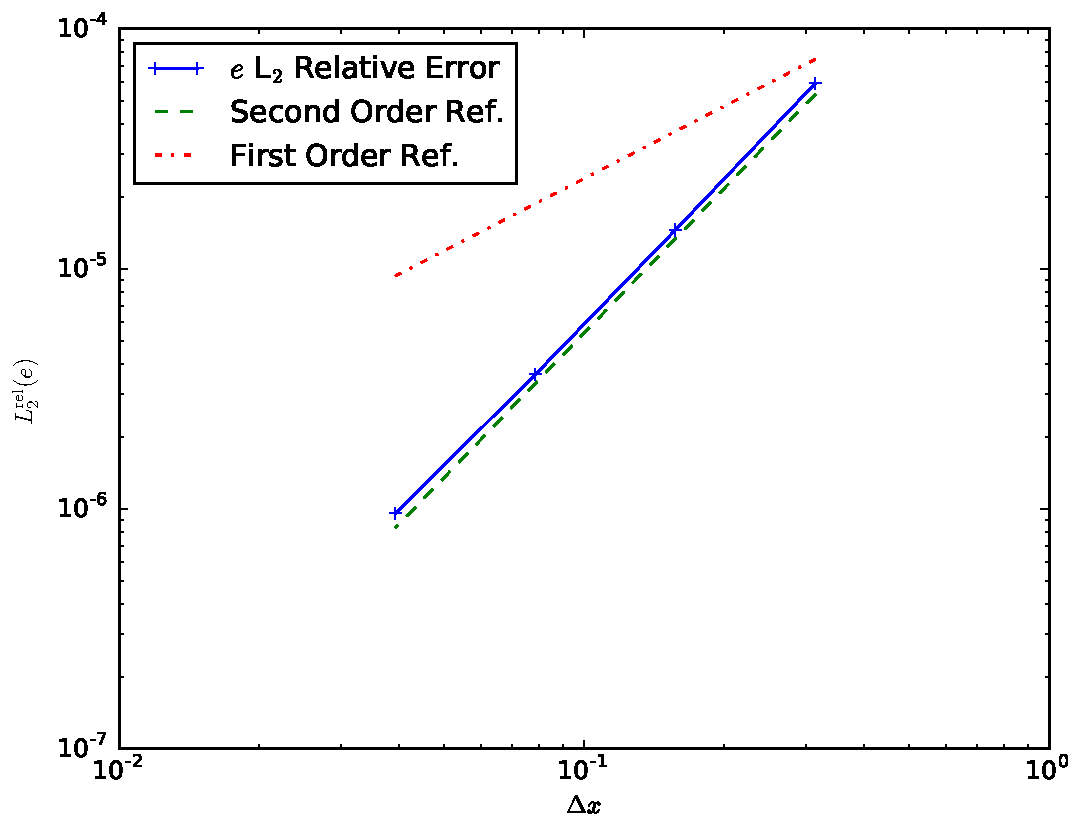
\includegraphics[width=\textwidth]{figures/MMS_diffusion_limit_e_convergence.pdf}
   \caption{Convergence of internal energy $e$ in space for the equilibrium diffusion limit MMS problem}
   \label{fig:diff_limit_e}
\end{figure}
\begin{figure}[ht]
   \centering
   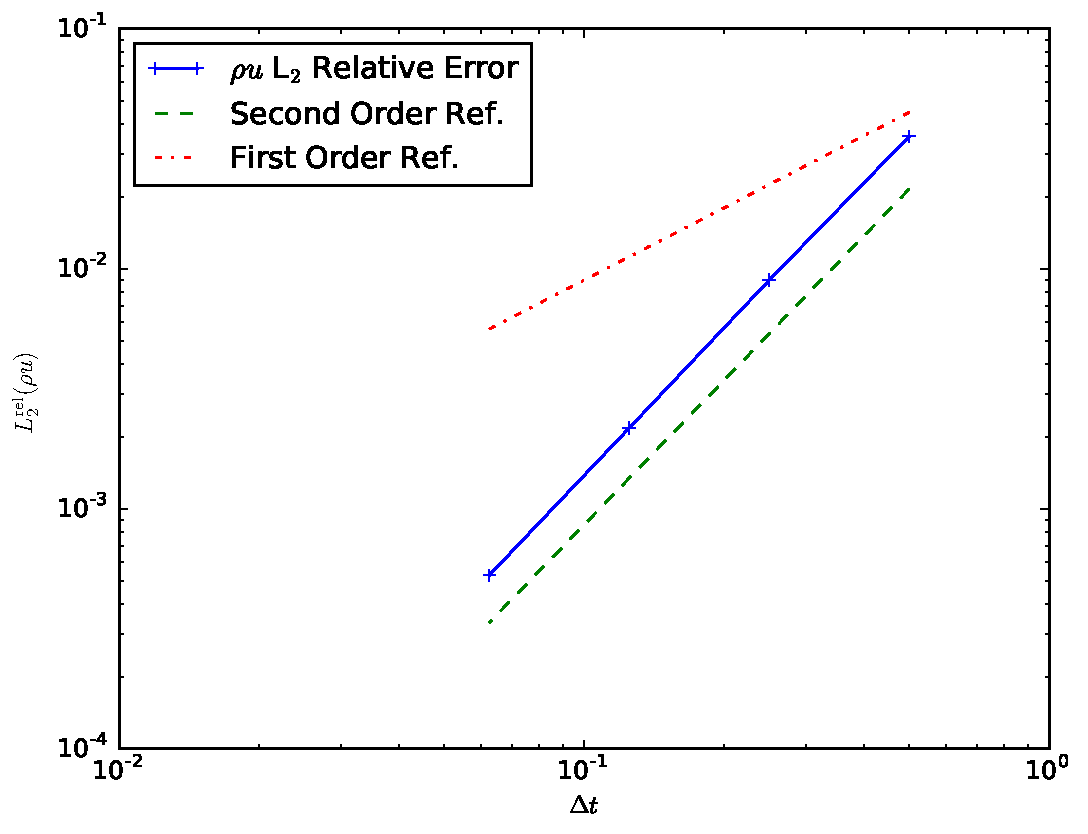
\includegraphics[width=\textwidth]{figures/MMS_diffusion_limit_rhou_convergence.pdf}
   \caption{Convergence of momentum $\rho u$ in time for the equilibrium diffusion limit MMS problem}
   \label{fig:diff_limit_mom}
\end{figure}

\subsection{Streaming Limit}

The second MMS problem corresponds to the streaming limit, in which the radiation
and hydrodynamics are weakly coupled. In this limit, radiation streaming dominates
relatively small radiation absorption and re-emission terms.  Here, we keep the re-emission term small by making the opacity
relatively small so that the radiation is nearly transparent to the fluid.  Also, because the radiation streams much faster than the fluid, this
results in a solution in which the unknowns evolve at significantly different time scales.  The functional form of the streaming solutions
are
\begin{subequations}
   \begin{equation} 
      \rho = \rho_{\infty}\left(\sin(x - t) + 2\right) \pec
   \end{equation} 
   \begin{equation}
       u = {a_{s\infty}} M\left(\cos(x - t) + 2\right) \pec 
   \end{equation} 
   \begin{equation} 
       p = \rho_\infty a_{s\infty}^2 \alpha\left(\cos(x - t) + 2\right) ,
   \end{equation}
    \begin{equation}
        \E = a T^4_{\infty}    \alpha\left(\cos(x - \mathbb{C}t) + 2\right) 
    \end{equation}
    \begin{equation}
        \F = a c T^4_{\infty} \alpha\left(\cos(x -  \mathbb{C}t) + 2\right) 
    \end{equation}
\end{subequations}
Here, was can see that the wave speed of the radiation energy density is faster than that of the hydrodynamic unknowns
by a factor of $\mathbb{C}$.  This solution is also defined to mimic an isothermal flow regime, in which the radiation
varies rapidly enough that changes in the fluid temperature are suppressed. In this case, the exact solution for the
fluid temperature is a constant.

All problem parameters are fixed and then the  space and time discretizations are refined uniformly.  The problem is fully defined
with the parameters $\mathbb{C}=100$, $\mathbb{P}=0.1$, $\rho_{infty}=1$ g cm$^{-3}$, $\gamma=5/3$, $\sigma_a=\sigma_t=1$ cm$^{-1}$,
$\alpha=0.5$ and $M=0.9$.  The relatively high value of $\mathbb{P}$ and low value of $\mathbb{C}$ produce a more
difficult problem to simulate, requiring convergence of the implicit solves. As before, the initial $\Delta
t$ is based on the Courant condition of 0.6. The simulation is performed until the initial radiation have advanced two periods, i.e., until
$t=4\pi/10$.

Figures~\ref{fig:streaming_e} and~\ref{fig:streaming_mom} plots the error convergence as a function of $\Delta x$ and $\Delta t$ for
internal energy and momentum, respectively.  
The convergence in the streaming
limit is closer to 1.8 for the momentum variable. A finer time step size may be required to resolve the radiation unknowns more accurately than the
Courant condition requires. The time step size may not yet be in the asymptotically converging region.

\begin{figure}[ht]
   \centering
   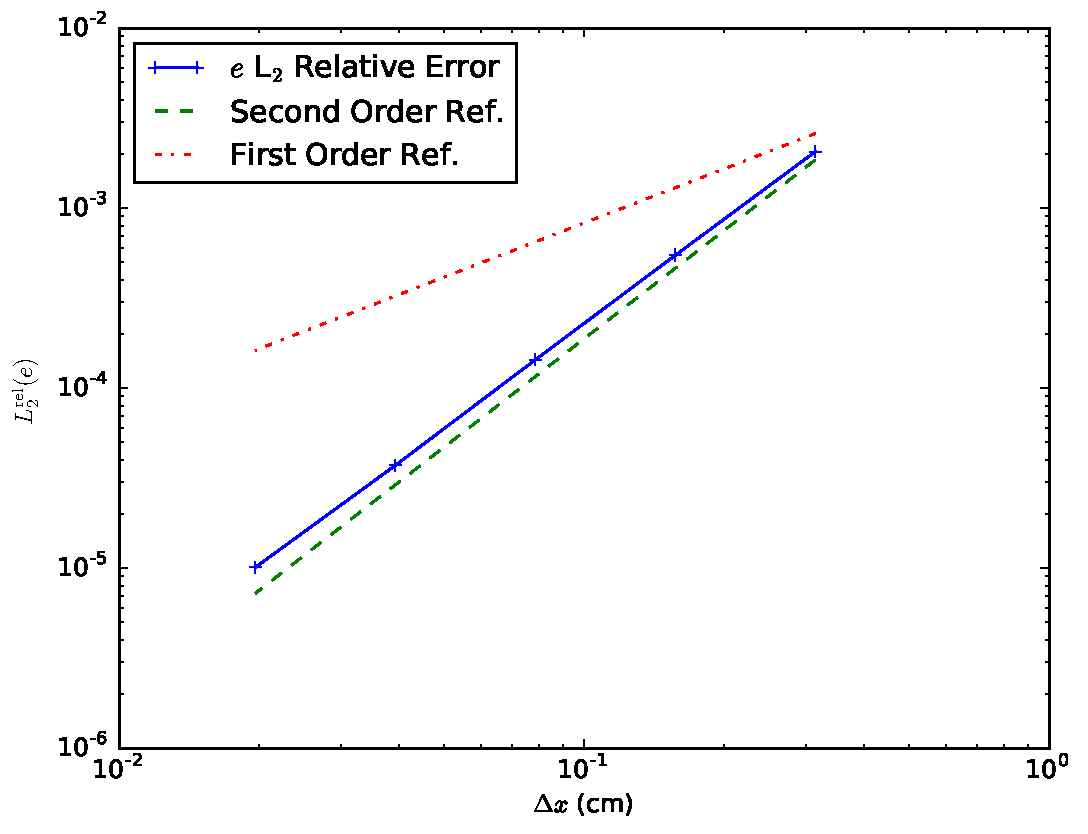
\includegraphics[width=\textwidth]{figures/MMS_streaming_e_convergence.pdf}
   \caption{\label{fig:streaming_e}Convergence of internal energy $e$ in space for the MMS streaming problem}
\end{figure}
\begin{figure}[ht]
   \centering
   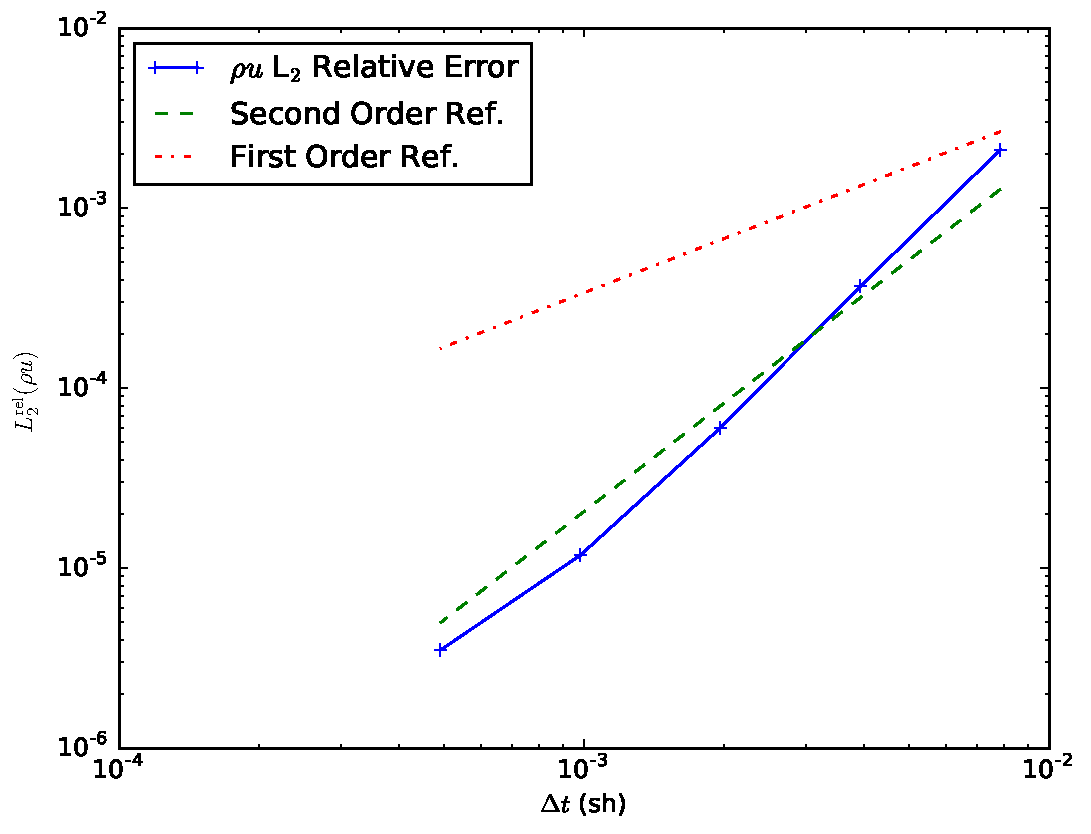
\includegraphics[width=\textwidth]{figures/MMS_streaming_rhou_convergence.pdf}
   \caption{\label{fig:streaming_mom}Convergence of momentum $\rho u$ in time for the MMS streaming problem}
\end{figure}


\section{Results for Radiation-Hydrodynamic Shocks}
\label{sec:ShockSolutions}

Reproducing radiative shocks accurately, particularly in the optically thick
regime, represents a challenging problem in the simulation of radiation
hydrodynamics. A numerical scheme must be able to meet these
challenges well.  We will compare simulated steady state, radiative shocks to semi-analytical solutions~\cite{jim???}. The
semianalytic solutions are based on a diffusion radiation model, which is equivalent to our S$_2$ radiation model at steady state.
To reduce simulation times, we initialize the shocks with the analytic steady state solution projected onto the cell centered meshes
and run the simulation until steady state is reached.
At the boundary, we compute the fluxes using our
standard Riemann solver, setting the hydrodynamic unknowns on the outside of the boundary equal to the far-stream conditions.  
Our algorithm will not be second-order globally due to the discontinuity at the shock~\cite{???}.  Thus, we are not interested in
order-accuracy here but are ensuring our code produce accurate solutions.
%We initialize each radiative shock calculation by setting the left half of the
%spatial domain equal to the far-upstream condition and the right half equal to
%the downstream condition. 

We test our algorithm for two radiative shocks, similar to those presented in
\cite{lowrie3}, which incorporate a variety of structural features.  For both shocks, we set $\gamma = 5/3$,
$c_v=0.14472799784454$ Jks keV$^{-1}$ g$^{-1}$ (1 Jk$=10^9$ J), and $\sigma_a = 577.35$ cm$^{-1}$. 
The problem specifications for the farstream pre and post-shock regions are provided in Table~\ref{tab:mach1.2_shock_IC}.
and Table~\ref{tab:mach3.0_shock_IC} for the Mach 1.2 and Mach 3 shock, respectively.
Results are generated with a CFL condition of 0.6 and $N_x=500$ spatial cells.

First, we compute the Mach 1.2 shock, which has a hydrodynamic shock but no
ISP.  Fig.~\ref{fig:mach1.2T} compare our
results with the semi-analytic solutions for the fluid and
radiation temperature.  We see good agreement between
the two.  In this solution, we see a discontinuity in both the density and
fluid temperature due to the hydrodynamic shock, and the maximum temperature is
bounded by the far-downstream temperature, since there is no ISP to drive it
further.


\begin{table}[ht]
  \centering
  \caption{Initial condition values for the Mach 1.2 radiative shock problem}
  \label{tab:mach1.2_shock_IC}
  \begin{tabular}{l l l l}\hline
      \emph{Parameter} & \emph{Pre-shock Value} & \emph{Post-shock Value} & \emph{Units}\\\hline
$\rho$ & 1.00000000e+00 & 1.29731782e+00 & g cm$^{-3}$ \\
$u$ & 1.52172533e-01 & 1.17297805e-01 & cm sh$^{-1}$ \\
$T$ & 1.00000000e-01 & 1.19475741e-01 & keV \\
$E$ & 2.60510396e-02 & 3.13573034e-02 & Jks cm$^{-3}$\\
$E_r$ & 1.37201720e-06 & 2.79562228e-06 & Jks cm$^{-3}$ \\
$F_r$ & 0.00000000e+00 & 0.00000000e+00 & Jks cm$^{-2}$ s$^{-1}$ \\
      \hline
  \end{tabular}
\end{table}
\begin{table}[ht]
  \centering
  \caption{Initial condition values for the Mach 3 radiative shock problem}
  \label{tab:mach3_shock_IC}
  \begin{tabular}{l l l l}\hline
      \emph{Parameter} & \emph{Pre-shock Value} & \emph{Post-shock Value} & \emph{Units}\\\hline
$\rho$ & 1.00000000e+00 & 3.00185103e+00 & g cm$^{-3}$ \\
$u$ & 3.80431331e-01 & 1.26732249e-01 & cm sh$^{-1}$ \\
$T$ & 1.00000000e-01 & 3.66260705e-01 & keV \\
$E$ & 8.68367987e-02 & 1.83229115e-01 & Jks cm$^{-3}$\\
$E_r$ & 1.37201720e-06 & 2.46899872e-04 & Jks cm$^{-3}$ \\
$F_r$ & 0.00000000e+00 & 0.00000000e+00 & Jks cm$^{-2}$ s$^{-1}$ \\
      \hline 
  \end{tabular}
\end{table}
\begin{figure}[ht!]
\centering
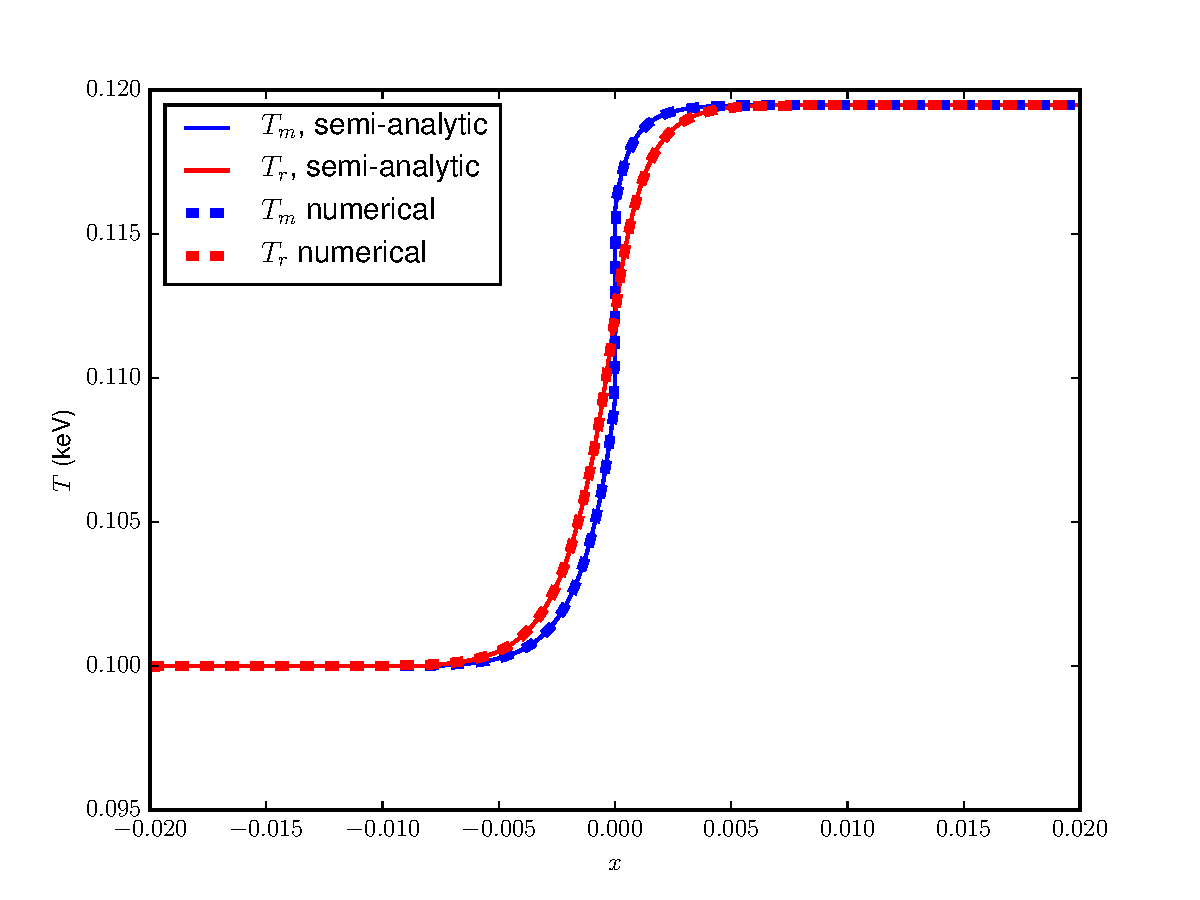
\includegraphics[width=\textwidth]{figures/radshock_mach_1_2.pdf}
\caption{\label{fig:mach1.2T}\bf Mach 1.2 radiative shock fluid and radiation temperatures.} 
\end{figure}

\begin{figure}[ht!]
\centering
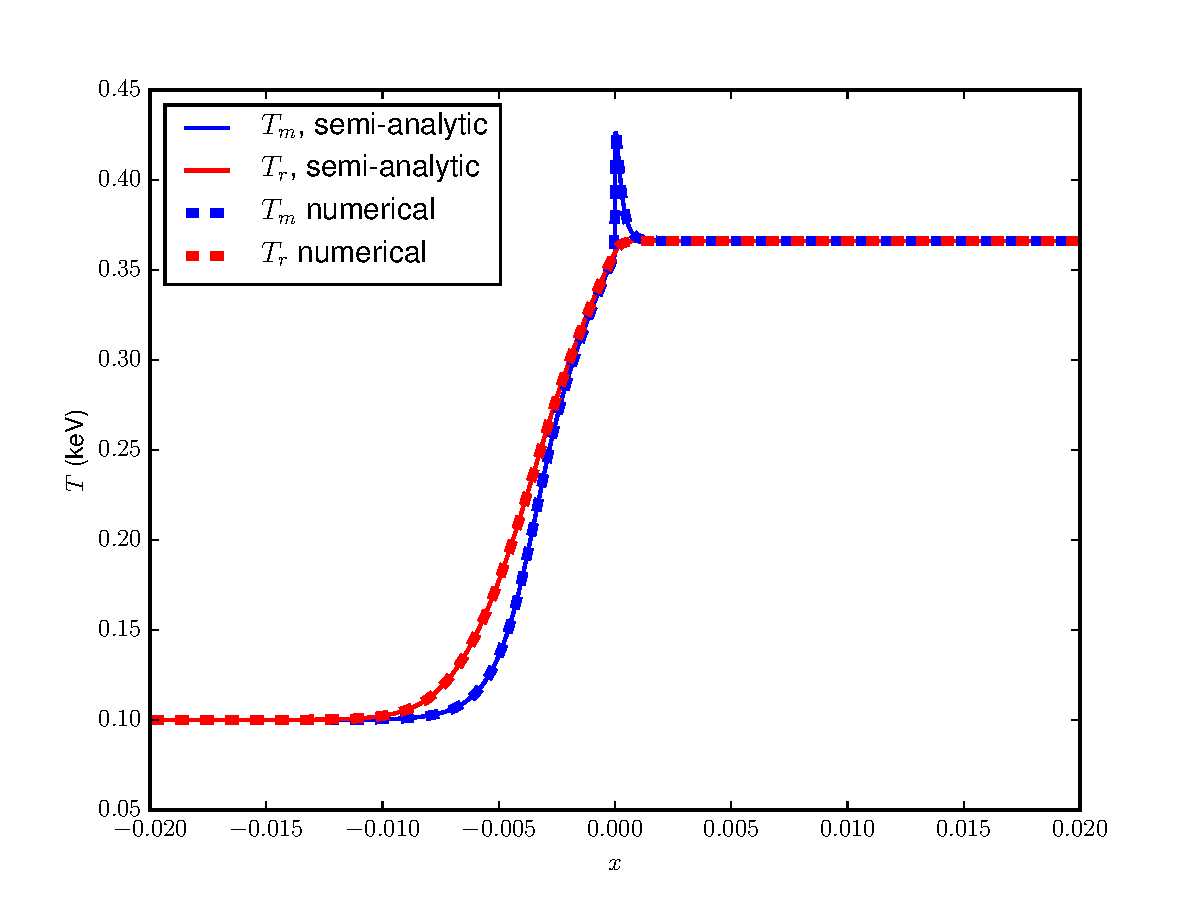
\includegraphics[width=\textwidth]{figures/radshock_mach_3_0.pdf}
\caption{\label{fig:mach3.0T}\bf Mach 3.0 radiative shock fluid and radiation temperatures.} 
\end{figure}


A Mach 3 shock is simulated that has both a hydrodynamic shock and an ISP.
Fig.~\ref{fig:mach3.0T} compares our numerical material and radiation temperature with the semi-analytic solutions.  In each of these
figures, we can see the effects of the hydrodynamic shock, causing a discontinuity in both the fluid density and
temperature.  We can also see the Zel'dovich spike, caused by the ISP embedded within the hydrodynamic shock, driving up
the fluid temperature at the shock front.  This spike leads to the relaxation region downstream as the fluid temperature
and radiation temperature equilibrate. Here, we can see that our results still show very good agreement with the semi-analytic solution.




\section{Conclusions and Future Work}
\label{sec:Conclusions}

We develop a new IMEX method for solving the equations of radiation-hydrodynamics that is second-order accurate in space
and time.  In addition to accuracy, we meet the goals outlined in Section \ref{sec:Introduction}: it reliably converges
non-linearities, rapidly damps oscillations, incorporates modern algorithms used by the hydrodynamics and radiation
transport communities, appears to have straightforward extensibility to a full radiation transport model, preserves the
diffusion limit in 1D in such a way that it is expected to preserve this limit in 2D and 3D, accurately computes
radiative shocks, and reduces to fundamental algorithms when the effects of coupled physics are negligible.  Thus, it
represents a very useful alternative to existing methods.

In future work, we recommend extending our radiation solver to incorporate a radiation transport model.  The structure
of our radiation-hydrodynamics algorithm should make this extension straightforward.  Since our algorithm only requires
the angle-integrated radiation energy density and radiation current, the radiation solver may, in some sense, be treated
as a black box module to compute these quantities.  Of course, the angular intensities will need to be preserved across
time steps. Momentum is already conserved by the chosen implicit statements.  It is likely not necessary to fully
converge the nonlinear solves in the predictor steps.


\bibliographystyle{model1-num-names}
\bibliography{References}


\clearpage

\appendix

%\section{Details of the Radiation-Hydrodynamics Method}
%Here we give a detailed description of our radiation-hydrodynamics method.
%First, we define some notation; the following are quantities stored
%throughout the calculation:
%\begin{center}
%\begin{tabular}{l|l}
%   Radiation angular intensities & $\R^n \equiv \{\Psi^\pm\iL,\Psi^\pm\iR\} \quad\forall i$ \\
%   Conservative hydrodynamics variables & $\H^n \equiv \{\rho_i^n, (\rho u)_i^n, E_i^n\} \quad\forall i$ \\
%   MHM fluid internal energy slopes & $\delta e^n \equiv \{\delta e_i^n\} \quad\forall i$ \\
%   MHM conservative variable slopes & $\bar{\Delta}^n \equiv \{\bar{\Delta}\rho_i^n, \bar{\Delta}(\rho u)_i^n,
%     \bar{\Delta} E_i^n\} \quad\forall i$ \\
%   Macroscopic cross sections & $\sigma^n \equiv \{\sigma_{s,i,L}^n, \sigma_{s,i,R}^n,
%   \sigma_{a,i,L}^n, \sigma_{a,i,R}^n, \sigma_{t,i,L}^n, \sigma_{t,i,R}^n\}
%   \quad\forall i$
%\end{tabular}
%\end{center}
%Other quantities are computed when needed.
%The solution for a time step $t^n\rightarrow t^{n+1}$ consists of four
%nonlinear solves:
%\begin{enumerate}
%  \item Backward-Euler step from $t^n$ to $t^{n+\fourth}$
%    (Cycle 1 Predictor)
%  \item Crank-Nicolson step from $t^n$ to $t^{n+\half}$
%    (Cycle 1 Corrector)
%  \item Backward-Euler step from $t^{n+\half}$ to $t^{n+\frac{3}{4}}$
%    (Cycle 2 Predictor)
%  \item TR/BDF-2 step from $t^{n+\half}$ to $t^{n+1}$
%    (Cycle 2 Corrector)
%\end{enumerate}
%
%\begin{enumerate}
%
%
%
%
%% Cycle 1 predictor
%
%\item \textbf{Perform Cycle 1 Predictor.} 
%\begin{enumerate}
%\item \textbf{Perform MUSCL-Hancock Predictor.} First, slopes $\Delta^n$ are
%computed via Equations \eqref{eq:muscl_slopes} and \eqref{eq:muscl_differences},
%optionally applying a slope limiter.
%Then a linear-discontinuous representation of the solution is created via
%Eq. \eqref{eq:edge_hydro}, and the
%the MUSCL-Hancock predictor is performed to obtain $\H^*$, the
%homogeneous hydrodyamics solution at $t^{n+\fourth}$,
%via Eq. \eqref{eq:muscl_predictor}.
%
%\item \textbf{Perform nonlinear iterations.} Iteration of the
%$t^{n+\fourth}$ solution is required since the system of equations
%is nonlinear. 
%\begin{enumerate}
%\item\label{item:vel_update}
%\textbf{Update velocities.} The Crank-Nicolson discretization
%of the velocity update equation, Eq. \requ{hydromCNfull},
%is solved to obtain new
%velocities at cell centers, $\{u_i^{k+1}\}$. Evaluation of
%the radiation quantities $\E$ and $\F$
%at cell centers is achieved by averaging the left and right values.
%
%\item \textbf{Update radiation.} The Crank-Nicolson discretization of the S-2
%equations, Equations \requ{S2CNfullL} and \requ{S2CNfullR} are solved,
%employing the linearization given in Section \ref{sec:linearization}.
%Evaluation of the densities and velocities at the edges is achieved using using
%the cell-centered values in conjunction with the slopes $\Delta^n$. Evaluation
%of the material energy $E$ at edges is achieved using the internal energy
%slopes $\delta e^n$ from a previous radiation solve.  The computation of this
%slope is described in Section~\ref{sec:e_slopes}.
%
%\item \textbf{Update internal energies.} The internal energies are
%updated in accordance with the linearization procedure given is Section
%\ref{sec:linearization}. The update equations produce edge values
%$\{e^{k+1}\iL,e^{k+1}\iR\}$. These left and right values are added to the 
%kinetic energy at edges to produce cell-averaged values for the total energy
%$\{E^{k+1}_i\}$, which are used in the subsequent iteration.  The values
%of $\delta e$ are stored for the next radiation solve.
%Cross sections that are updated if they are functions of the hydrodynamic 
%state of the fluid.
%
%\end{enumerate}
%\end{enumerate}
%
%% Cycle 1 corrector
%
%\item \textbf{Perform Cycle 1 Corrector.} This step proceeds
%just as the predictor step, except that the MUSCL-Hancock
%corrector step given by Eq. \eqref{eq:muscl_corrector} is used instead of the MUSCL-Hancock predictor
%step, and the step goes from $t^n$ to $t^{n+\half}$ instead
%of $t^n$ to $t^{n+\fourth}$. No new hydrodynamic slopes are computed;
%evaluation of edge densities and velocities use
%$\Delta^n$.  However, evaluation of edge internal energies
%in the nonlinear iteration use $\delta e^{n+1/4}$. At the end
%of the cycle, the new internal energy slopes $\delta e^{n+\half}$
%are saved for the next cycle.
%
%% Cycle 2 predictor
%
%\item \textbf{Perform Cycle 2 Predictor.} This step proceeds
%just as the Cycle 1 predictor step, except that the
%step goes from $t^{n+\half}$ to $t^{n+\frac{3}{4}}$ instead
%of $t^n$ to $t^{n+\fourth}$. As in Cycle 1, new slopes
%are computed in the MUSCL-Hancock predictor step;
%these slopes $\Delta^{n+\half}$ are then used for
%evaluation of edge densities and velocities in the remainder
%of the cycle. Evaluation of edge internal energies
%and temperatures use the internal energies saved
%from the end of Cycle 1, $\delta e^{n+\half}$.
%
%% Cycle 2 corrector
%
%\item \textbf{Perform Cycle 2 Corrector.} This step proceeds
%as the Cycle 1 corrector step, except that the time step goes
%from $t^{n+\half}$ to $t^{n+1}$, and the time discretization
%of the equations is a form of TR/BDF-2
%instead of Crank-Nicolson, so values at $t^n$
%are used in the temporal discretization. Slopes
%$\Delta^{n+\half}$ and $\delta e^{n+\frac{3}{4}}$  are again
%used to evaluate edge quantities. At the end
%of the cycle, the new internal energy slopes $\delta e^{n+1}$
%are saved for the next cycle.
%
%% End
%
%\item \textbf{Store values for next time step.}
%At this point, the old solutions, hydrodynamics slopes,
%internal energy slopes, and cross sections
%are saved for the next time step.
%
%\end{enumerate}

%===============================================================================
\section{The Time-Discretized Equations}\lsec{full}

In this section, we detail each of the equations for the MHM and iterative radiation
solves.  The radiative transfer and hydrodynamic operators are treated independently via
operator-splitting.  Within the predictor and corrector stage of each cycle, there is an explicit hydrodynamic solve, followed by an associated implicit radiation solve. 
We will use a $*$ superscript to denote the intermediate operator-splitting states of variables resulting
from the hydrodynamic steps. 


%===============================================================================
%===============================================================================
\subsection{The MUSCL-Hancock Method}
%================================================================== 

The MHM handles the fluid advection portion of the RH equations by advancing the homogeneous Euler equations
in time.   The homogeneous Euler equations may be expressed in conservative form as
\begin{equation}
  \dydt{\H} + \nabla\cdot\Flux(\H) = \mathbf{0} \pec
\end{equation}
where $\H$ is a vector of the conservative unknowns
and $\Flux(\H)$ is the flux associated with each, i.e.,
\begin{equation}
  \H=\left[\begin{array}{c}\rho\\\rho u\\E\end{array}\right] \pec\qquad
  \Flux(\H)=\left[\begin{array}{c}\rho u\\
  \rho u^2 + p\\
  (E+p)u\end{array}\right] \pep
\end{equation}
Each cycle consists of a MHM predictor and corrector stage. For example, the first predictor step advances the hydrodynamic unknowns
from $H^{n}$ to $H^{*n+1/4}$.
The predictor step begins by constructing a cell-wise linear representation of the solution
using reconstructed slopes $\Delta_i^n$:
\begin{equation}\label{eq:muscl_slopes}
  \Delta_i^n = \half\left(\Delta\H_{i-\half}^n + \Delta\H_{i+\half}^n\right) \pec
\end{equation}
\begin{equation}\label{eq:muscl_differences}
  \Delta\H_{i-\half}^n = \H_i^n - \H_{i-1}^n \pec\quad
  \Delta\H_{i+\half}^n = \H_{i+1}^n - \H_i^n \pec
\end{equation}
The slopes are modified using a double-minmod slope
limiter to ensure positivity and stability~\cite{mclow2008}.
A linear representation
of the solution within each cell is then constructed as
\begin{equation}\label{eq:edge_hydro}
  \H\iL^n = \H_i^n - \frac{{\Delta}_i^n}{2} \pec
  \quad
  \H\iR^n = \H_i^n + \frac{{\Delta}_i^n}{2} \pec
\end{equation}
This representation is then evolved by a quarter of a time step:
\hydroPredictor{n}{*n+\fourth}{\fourth}{\label{eq:muscl_predictor}}

At this point, an implicit Euler radiation solve advances the system from $t^{*n+\fourth}$
to $t^{n+\fourth}$, as detailed in Sec.~\ref{}.  Then, the corrector step of the
MUSCL-Hancock method is applied.  The corrector step employs an approximate Riemann solver
to compute the fluxes based on the predicted hydrodynamic variables, i.e.,
\hydroCorrector{n}{n+\fourth}{*n+\half}{2}{\label{eq:muscl_corrector}}
where the fluxes are computed using an HLLC approximate Riemann solver~\cite{toro}.  At
each edge, the Riemann solver uses linearly extrapolated values, based on lagged
hydrodynamic slopes.  For example, at the edge
$x_{i-\half}$, the Riemann solver computes fluxes with the states
$\H_{i}^{n+1/4}-\frac{\Delta_i^n}{2}$ and $\H_{i-1}^{n+\fourth}+\frac{\Delta_{i-1}^n}{2}$.
The predictor and corrector steps for the second cycle proceed in the same manner.

\subsection{The Iterative Radiation Solves}

During each implicit radiation solve, the momentum deposition due to radiation and the
energy exchange due to black-body emission must be iteratively solved.  An outer fixed-point
iteration is performed for the velocity update.  Within each outer iteration, an analytic
Newton step is taken for the radiative transfer terms.  The iterations are repeated until 
convergence.  The equations below are for the $k+1$-st iteration within
each stage of the algorithm. 

\subsubsection{Velocity Update Equation}

During the iteration loop, a lagged estimates of the radiation unknowns are used to compute a new
material velocity.  The discretization of the radiation equations produces a linear
solution within a cell, which is represented with edge unknowns, e.g., $\E_{L,i}$ and
$\E_{R,i}$.  The edge values for radiation momentum deposition are spatially averaged to update the cell-averaged material
velocity.  
The BDF2 discretization of the velocity update equation for the cycle 2 corrector
step is
\momentumUpdateBDFTwo{n}{n+1/2}{2}{_i}{n+1}{\lequ{hydromBDF2full}}
where the $*$ terms came from the MHM corrector stage.  The cell-averaged terms on the right hand side are are computed by taking the linear
average of the corresponding expressions evaluated at the edges, e.g., 
\begin{multline}
   \left[\frac{\sigma_t}{c}\left(\F - \frac{4}{3}\E u\right)\right]_i =
   \half\left[\frac{\sigma_{t,i,L}}{c}\left(\F\iL - \frac{4}{3}\E\iL u\iL\right)\right]\\
   + \half\left[\frac{\sigma_{t,i,R}}{c}\left(\F\iR - \frac{4}{3}\E\iR u\iR\right)\right]
   \pep
\end{multline}
It is noted that in the absence of an extraneous momentum source, $\rho^{*n+1}=\rho^{n+1}$. In the
presence of MMS sources, $\rho$ is updated prior to entering the iteration loops.
The Crank-Nicolson discretization of the velocity update equation for the Cycle 1
corrector is
\momentumUpdateCN{n}{2}{_i}{n+1/2}{\lequ{hydromCNfull}}
The Backward-Euler discretization of the velocity update for the predictor stages are analogously defined.

\subsubsection{Radiation and Material Energy Equations}

The radiation and material energy equations must be linearized to be solved.  We use
a standard Newton linearization, with temperature dependent material properties lagged one
iteration~\cite{morelldsn}.  Upon linearization, the radiation unknowns can be directly
determined, followed by solution for new internal energies.  The linearization process is
tedious but straight forward.  For brevity, we provide the non-linear equations here.

With the updated momentum, a kinetic energy can be defined, allowing for new internal
energies to be obtained.  However, to simultaneously solve the radiation and material energy balance equations,
hydrodynamic quantities need to be evaluated at cell edges. The slopes $\Delta_i$
evaluated during the predictor step of the cycle, as given in Eq.~\eqref{eq:muscl_slopes}, are used
to extrapolate edge quantities during that cycle.  Evaluation of edge
densities is achieved by applying the slopes as given by Eq. \eqref{eq:edge_hydro}:
\begin{equation}
   \rho\iL^k = \rho_i^k - \frac{\Delta\rho_i^n}{2} \pep
\end{equation}
Evaluation of edge velocities is
achieved based on $\rho$ and $\rho u$ at edges, e.g.,
\begin{equation}
   u\iL^k = \frac{(\rho u)\iL^k}{\rho\iL^k}
          = \frac{(\rho u)_i^k - \frac{\Delta(\rho u)_i^n}{2}}
                 {\rho_i^k - \frac{\Delta\rho_i^n}{2}} \pep
\end{equation}
As explained in Section~\ref{sec:e_slopes}, internal energy unknowns, and thus material
temperature, use slopes that are independent of the MUSCL-Hancock slopes.  This modifies
the $E^*$ terms within a cycle.
These radiation internal energy slopes are denoted by $\delta e$. Evaluation
of edge internal energies is thus performed as follows:
\begin{equation}
   e\iL^k = e_i^k - \frac{\delta e_i^n}{2} \pep
\end{equation}
 These internal energy slopes are only updated at the end of each stage, i.e.,
when the nonlinear iteration for the corrector step have been converged.

With hydrodynamic variables defined, discretized equations for the radiation and material
energy balance equations can be defined.
A lumped linear discontinuous (LLDG) spatial discretization is employed
for the S$_2$ equations~\cite{???}.  The lumping of the equations produces strictly
positive intensities in
1D~\cite{???}. Standard upwinding is used to define face terms in the spatial gradient term for the radiation equations.  
For reference, the radiation equation for
the positive direction of flow, the left unknown, and the first Backward-Euler stage is
\begin{equation}
\lequ{S2BEfullL}\begin{split}
  \frac{4}{c}\frac{\psi\iL^{+,n+1/4,k+1}-\psi\iL^{+,n}}{\dt} = &
  -\frac{2\mu^+}{h_i}\fn{\psi^{+,n+\fourth,k+1}_i - \psi^{+,n+\fourth,k+1}_{R,i-1}}
   -\half\sigma_{t,i,L}^k\psi\iL^{+,k+1}\\
   & +\frac{\sigma_{s,i,L}^k}{2}\phi\iL^{n+\fourth,k+1} +\half\sigma_a a c
   \left(T_{i,L}^{n+1/4,k+1}\right)^4
   \pep
\end{split}
\end{equation}
where $\psi_{i}^+ = (\psi_{i,L}^+ + \psi_{i,R}^+)/2$.  The corresponding equation
for the right unknown is
\begin{equation}
    \lequ{S2BEfullR}\begin{split}
  \frac{4}{c}\frac{\psi\iR^{+,n+1/4,k+1}-\psi\iR^{+,n}}{\dt} = &
  -\frac{2\mu^+}{h_i}\fn{\psi^{+,n+\fourth,k+1}_{i,R} - \psi^{+,n+\fourth,k+1}_{i}}
   -\half\sigma_{t,i,R}^k\psi\iR^{+,k+1}\\
   & +\frac{\sigma_{s,i,L}^k}{2}\phi\iR^{n+\fourth,k+1} +\half\sigma_a a c
   \left(T_{i,R}^{n+1/4,k+1}\right)^4
   \pep
\end{split}
\end{equation}
For 1D, the $S_2$ equations can be
directly solved efficiently.     

The material energy balance equations are also discretized in space to determine new edge
values. 
The Crank-Nicolson discretization of the material energy balance equation for the $L$
unknowns is
\energyUpdateCN{n}{}{\iL}{n+1/2}{\lequ{hydroECNfull}}
The BDF2 discretization of the energy update equation is
\energyUpdateBDFTwo{n}{n+1/2}{}{\iL}{n+1}{\lequ{hydroEBDF2full}}
To conserve total energy, the newly estimated edge total
material energies, $E_{L,i}^{k+1}$ and $E_{R,i}^{k+1}$, are averaged to compute new
cell-averaged total energies $E_{i}^{k+1}$; no modifications are made to the hydrodynamic slopes
$\Delta_i$.  Averaging the total energy in this manner produces an unavoidable discrepancy between cell-averaged and edge
internal energies. 

\subsection{Using Radiation Internal Energy Slopes}
\label{sec:e_slopes}

As discussed in the introduction, the radiation solver and hydro solver use different
internal energy slopes as an approach to preserve the equilibrium diffusion limit.   The
implementation of separate slopes is a proof of concept for higher dimensions.
To mitigate confusion, in this section we will denote the hydro-state internal energy variables as $e$ and
the internal energy variables coming from the non-linear radiation solves as $e^r$. Care must be taken to
ensure that total energy is conserved.  The modified slopes are only applied to the implicit terms in each
nonlinear solve.

During the MHM solve, we
use the standard slope reconstruction formulas to advect variables to
state $U^*$ (or $U^{**}$), including total energy $E$.  Then, in the non-linear iteration loop for the radiation
and internal energy densities we use a modified slope for $E^*$, denoted $\Delta E^{r*}$, that will preserve the diffusion
limit.  This $\Delta E^{r*}$ is based on the edge values of $e^r$ of \emph{the last iteration of the previous
nonlinear radiation solve}.  For example, if we are solving the cycle 1 corrector from state $e^*$ to
$e^{n+1/2}$, we use the edge values of $e^r$ from the last iteration of the solve for
$e^{r,n+1/4}$ to construct the slopes for $\Delta E^{r,*}$. The value of $\Delta
E^{r,*}$ does not change over the duration of the nonlinear solve.

Slopes
$\Delta^{n+\half}$ and $\delta e^{n+\frac{3}{4}}$  are again
used to evaluate edge quantities. At the end
of the cycle, the new internal energy slopes $\delta e^{n+1}$
are saved for the next cycle.


For the nonlinear solve we need the to use $\delta e^r$ to construct
$\Delta E^{*r}$ in the next solve (and thus the values $E^*_{R/L} = E^*_i \pm \frac{1}{2}\Delta E^{r*}$
needed for the LD radiation solve).  We approximate this slope based on the hydro values
for $E^*$ as:
\begin{equation}
    \Delta E^{r*} = E^{r*}_R - E^{r*}_L
\end{equation}
where 
\begin{equation}\label{estarr}
    E^{r*}_R = \rho^*_R\left((u_R^*)^2 + e^*_i +
    \delta e^{r,n+1/4}\right),
\end{equation}
\begin{equation}\label{estarl}
    E^{r*}_L = \rho^*_R\left((u_L^*)^2 + e^*_i -
    \delta e^{r,n+1/4}\right),
\end{equation}
and subscript $i$ denotes cell average quantities.  The edge values of $\rho$ and
$u$ are evaluated using the MHM slopes as usual.
 Once we have completed
the nonlinear solve for $e^{r,n+1/2}_{L/R}$, we must compute the change made to the
cell-averaged total energy for the next MHM solve, such that total energy is conserved. The formula for the new total energy is
\begin{equation}\label{ei}
    E^{n+1/2}_i = \frac{1}{2}\left[\rho_L\left(\frac{1}{2}u_L^2 + e_L^r\right)
    +\rho_R\left(\frac{1}{2}u_R^2 + e_R^r\right)\right]^{n+1/2}
\end{equation}
where all variables are at time $t^{n+1/2}$. The internal energy slopes are computed
and stored for the next nonlinear solve.  For the first solve, the internal energy
slopes are assumed zero.

%%===============================================================================
%\subsection{Linearization of Equations for General Temporal Discretization}
%%===============================================================================
%\label{sec:linearization}
%Within each solution time step, first the hydro variables are advected (either
%using local predicted fluxes or a Riemann solver).  Then, a non-linear system
%must be solved iteratively with iteration index $k$.  Consider the case of a non-linear system over a single step from
%$t_n$ to $t_{n+1}$. We will combine all known source terms as $Q_k$, which are known from previous states in time or
%the previous iteration $k$.  To linearize the system, we perform the standard
%approach of linearizing the Planckian function about some temperature near
%$T^{n+1}$, denoted $T^k$. For the initial iteration, $T^k=T^n$.  
%
%First, the original equation is rewritten as
%\begin{align*}
%   \frac{E^{k+1} - E^*}{\dt} &= - \alpha \left[\sa^k c \left(
%   a(T^{k+1})^4 - \E^{k+1}\right)\right]+Q_E^k \\
%\end{align*}
%where for BDF2,
%\begin{multline}
%    Q^{k}_E = -\frac{1}{6}\left[\sa c\left( aT^4 - \E\right)\right]^{n-1}
%    -\frac{1}{6}\left[\sa c\left( aT^4 - \E\right)\right]^{n} \\
%    +\BDF{\sigma_t \frac{u}{c} \left( \F - \frac{4}{3} \E u \right)}{n-1}{n}{k},
%\end{multline}
%for CN,
%\begin{multline}
%    Q^{k}_E = -\half\left[\sa c\left( aT^4 - \E\right)\right]^n\\
%   +\CN{\sigma_t \frac{u}{c} \left( \F - \frac{4}{3} \E u \right)}{n}{k},
%\end{multline}
%and for BE,
%\begin{equation*}
%    Q^{k}_E = \sigma_t \frac{u}{c} \left( \F - \frac{4}{3} \E u \right)^k.
%\end{equation*}
%The scale factor $\alpha$ for BE, CN, and BDF2 is 1, $\half$, and $\frac{2}{3}$,
%respectively.  With these definitions, the Planckian source term becomes
%\begin{multline}
%   \sigma_a^k a c\left(T^{k+1}\right)^4 = \left(1 - \nu_{\alpha}^k\right)
%   \sigma_a^k a c (T^k)^4 + \sigma_a^k c \nu_{\alpha}^k \E^{k+1}\\
%   +\frac{\nu_{\alpha}^k}{\alpha} Q_E^k - \frac{\rho\nu_{\alpha}^k}{\alpha\dt}
%   \left[(e^k - e^*) + \frac{1}{2}((u^{k+1})^2 - (u^*)^2)\right] \pep
%\end{multline}
%with 
%\begin{equation}
%    \nu^k_{\alpha} = \frac{\alpha\sigma_a c\Delta t \frac{\beta^k}{\rho}}{1 +
%    \alpha\sigma_a c\Delta t \frac{\beta^k}{\rho}}.
%\end{equation}
%and $\beta^k=\frac{4a(T^k)^3}{c_v^k}$.
%The energy update equation becomes
%\begin{multline}
%    \label{eq:energy_update}
%    e^{k+1} = \alpha\frac{(1-\nu_{\alpha})\Delta t}{\rho}\left[\sigma_a^k c \left(
%    \E^{k+1} - a(T^k)^4\right) + \frac{Q_E^k}{\alpha} \right] \\ - (1 -
%    \nu_{\alpha})\left(\frac{1}{2}[(u^{k+1})^2 - (u^*)^2]\right)
%    +(1-\nu_\alpha)e^*+ \nu_{\alpha}e^k \pep
%\end{multline}
%After solving for $\E^{k+1}$, a new internal energy can be estimated
%using Eq.~\eqref{eq:energy_update} to conserve energy.  Momentum is only conserved to
%the tolerance of the velocity iterations.  
%Iterations are repeated until
%convergence, beginning with a solve of Eq.~\eqref{eq:vel_update} with updated
%radiation quantities.  Once the system is converged, the EOS can be used to
%update $p^{n+1}$.

%%===============================================================================
%\section{Conservation}
%%===============================================================================
%In the homogeneous hydrodynamics case (where there is no coupling to radiation),
%one can arrive at a conservation statement for a time step for each conserved
%quantity $H$ by summing the MUSCL-Hancock update equation, Eq.
%\eqref{eq:muscl_corrector}, multiplied by cell volume $h_i$, for all elements:
%\begin{equation}
%   \sum\limits_i h_i H_i^* = \sum\limits_i h_i H_i^n
%   + \Delta t^n\left(F_{\half}^{H,n+\half} - F_{N+\half}^{H,n+\half}\right) \pep
%\end{equation}
%The conservation statement for the momentum source update, obtained for
%Crank-Nicolson by summing Eq. \eqref{eq:hydromCNfull} multiplied by cell
%volume $h_i$ for all elements, is
%\begin{equation}
%   \sum\limits_i h_i \rho_i^* u_i^{k+1} = \sum\limits_i h_i (\rho u)_i^*
%   +\dt^n\left(
%   \half\sum\limits_i h_i \frac{\sigma_{t,i}^n}{c}\F_{0,i}^n
%   + \half\sum\limits_i h_i \frac{\sigma_{t,i}^n}{c}\F_{0,i}^k
%   \right) \pep
%\end{equation}
%The conservation statement for the radiation momentum is obtained by
%manipulating the discretized S-2 equations:
%\begin{multline}
%   \sum\limits_i h_i \frac{\F_i^{k+1}}{c^2} = \sum\limits_i h_i \frac{\F_i^n}{c^2}
%   + \dt^n\Bigg(
%   \half\frac{1}{3c}\fn{\Psi^{+,n}_{inc} - \Psi^{-,n}_{inc}
%   + \Psi^{-,n}_{1,L} - \Psi^{+,n}_{N,R}}\\
%   + \half\frac{1}{3c}\fn{\Psi^{+,k+1}_{inc} - \Psi^{-,k+1}_{inc}
%   + \Psi^{-,k+1}_{1,L} - \Psi^{+,k+1}_{N,R}}\\
%   - \half\sum\limits_i h_i\fn{\half\frac{\sigma_{t,i,L}^n}{c}\F_{0,i,L}^n
%   + \half\frac{\sigma_{t,i,R}^n}{c}\F_{0,i,R}^n}\\
%   - \half\sum\limits_i h_i\fn{\half\frac{\sigma_{t,i,L}^k}{c}\F_{0,i,L}^{k+1}
%   + \half\frac{\sigma_{t,i,R}^k}{c}\F_{0,i,R}^{k+1}}
%   \Bigg) \pep
%\end{multline}
%Combining this with the hydrodynamics momentum conservation statement
%gives the total momentum conservation statement for Crank-Nicolson:
%\begin{multline}
%   \sum\limits_i h_i\fn{\rho_i^* u_i^{k+1} + \frac{\F_i^{k+1}}{c^2}} =
%   \sum\limits_i h_i\fn{\rho_i^* u_i^n + \frac{\F_i^n}{c^2}}\\
%   + \dt^n\bigg(
%   F_{\half}^{n+\half} - F_{N+\half}^{n+\half}
%   + \half\frac{1}{3c}\fn{\Psi^{+,n}_{inc} - \Psi^{-,n}_{inc}
%   + \Psi^{-,n}_{1,L} - \Psi^{+,n}_{N,R}}\\
%   + \half\frac{1}{3c}\fn{\Psi^{+,k+1}_{inc} - \Psi^{-,k+1}_{inc}
%   + \Psi^{-,k+1}_{1,L} - \Psi^{+,k+1}_{N,R}}
%   \bigg) \pep
%\end{multline}
%It is noted that if one is interested in checking the radiation momentum balance for
%a problem with no fluid motion (thermal radiative transfer only), then there is
%the extra momentum deposition terms that do not cancel out in the $S_2$ equations
%that must be accounted for.  To include MMS sources, the hydro sources can be added directly.  The radiation
%sources must also be included in the momentum.  The moments of the extra source are taken in the same way
%as they are for arriving at the radiation balance equation, resulting in an extra
%term of $\frac{1}{2c}[\mu^+(Q_L^+ + Q_R^+) - \mu^-(Q_L^- + Q_R^-)]$ to be added to
%the balance.
















\end{document}






%% The Appendices part is started with the command \appendix;
%% appendix sections are then done as normal sections
%% \appendix

%% \section{}
%% \label{}

%% References
%%
%% Following citation commands can be used in the body text:
%% Usage of \cite is as follows:
%%   \cite{key}          ==>>  [#]
%%   \cite[chap. 2]{key} ==>>  [#, chap. 2]
%%   \citet{key}         ==>>  Author [#]

%% References with bibTeX database:

\bibliographystyle{model1-num-names}
\bibliography{References}

%% Authors are advised to submit their bibtex database files. They are
%% requested to list a bibtex style file in the manuscript if they do
%% not want to use model1-num-names.bst.

%% References without bibTeX database:

% \begin{thebibliography}{00}

%% \bibitem must have the following form:
%%   \bibitem{key}...
%%

% \bibitem{}

% \end{thebibliography}


\end{document}

%%
%% End of file `elsarticle-template-1-num.tex'.
